\documentclass[a4paper,12pt]{article}

% PACKAGES
\usepackage[T1]{fontenc}
\usepackage[utf8]{inputenc}
%\usepackage{lmodern}
\usepackage[french]{babel}
\usepackage{csquotes}
\usepackage[notes,backend=biber]{biblatex-chicago}
\bibliography{biblio/mabiblio.bib}
\usepackage{amsmath}
\usepackage{amssymb}
\usepackage{amsthm}
\usepackage{amscd}
\usepackage{lmodern}
\usepackage{textcomp}
\usepackage{graphicx}

% MISE EN PAGE
\setlength{\voffset}{-3.75cm}
\setlength{\hoffset}{-2.6cm}
\setlength{\oddsidemargin}{2.5cm} % OBLIGATOIRE
\setlength{\evensidemargin}{2.5cm} % OBLIGATOIRE
\setlength{\topmargin}{2.5cm} % OBLIGATOIRE !!!
\setlength{\headheight}{0in}
\setlength{\headsep}{0in}
\setlength{\topskip}{0in}
\setlength{\parindent}{0cm}
\setlength{\parskip}{1ex plus0.4ex minus0.2ex}
\setlength{\textwidth}{16cm} % OBLIGATOIRE
\setlength{\textheight}{24.7cm} % OBLIGATOIRE
\renewcommand{\baselinestretch}{1.5} % OBLIGATOIRE
\flushbottom
\setcounter{page}{1}
\setcounter{tocdepth}{4}
\usepackage{helvet} % OBLIGATOIRE
\renewcommand{\familydefault}{\sfdefault} % OBLIGATOIRE

% PERSO
\newcommand{\guill}[1]{«~#1~»}
\newcommand{\eme}[0]{$^\text{e}$}
\newcommand{\Ier}[0]{I$^\text{er}$} \newcommand{\IIe}[0]{II\eme} \newcommand{\IIIe}[0]{III\eme} \newcommand{\IVe}[0]{IV\eme} \newcommand{\Ve}[0]{V\eme} \newcommand{\VIe}[0]{VI\eme} \newcommand{\VIIe}[0]{VII\eme} \newcommand{\VIIIe}[0]{VIII\eme} \newcommand{\IXe}[0]{IX\eme} \newcommand{\Xe}[0]{X\eme} \newcommand{\XIe}[0]{XI\eme} \newcommand{\XIIe}[0]{XII\eme} \newcommand{\XIIIe}[0]{XIII\eme} \newcommand{\XIVe}[0]{XIV\eme} \newcommand{\XVe}[0]{XV\eme} \newcommand{\XVIe}[0]{XVI\eme} \newcommand{\XVIIe}[0]{XVII\eme} \newcommand{\XVIIIe}[0]{XVIII\eme} \newcommand{\XIXe}[0]{XIX\eme} \newcommand{\XXe}[0]{XX\eme} \newcommand{\XXIe}[0]{XXI\eme}
\newcommand{\bigO}[1]{\mathcal O\left( #1 \right)}
\newcommand{\bigOmega}[1]{\Omega\left( #1 \right)}
\newcommand{\bigTheta}[1]{\Theta\left( #1 \right)}
\newcommand{\zitat}[2]{\#Citation(#2)\#}
\newcommand{\maze}[0]{\emph{m\symbol{64}ze\textdegree2}}
\newcommand{\tpp}[0]{[\dots]}










\title{\Large Internship report \\ \LARGE Computational analysis of jazz chord sequences}
\author{\normalsize Romain \textsc{Versaevel}, M1 Informatique Fondamentale, ENS de Lyon\\
\normalsize Tutored by David \textsc{Meredith}, Associate Professor, Aalborg University,\\
\normalsize leader of the Music Informatics and Cognition group\\}
\date{\today}

\begin{document}

\maketitle
\newpage

\tableofcontents

\newpage

\section{Introduction}

\section{Enjeux et présentation}

\subsection*{Enjeux}

\zitat{L'ordinateur, pendant longtemps, a été la seule vitrine de l'informatique aux yeux du grand public. Chacun sait mieux maintenant que ce domaine comporte de multiples dimensions : les enjeux industriels, l'univers complexe de la programmation et des langages, les foisonnements des différents usages, mais aussi l'affirmation que la logique et une certaine forme de rationalité dont désormais partie de notre culture contemporaine \tpp~
Désormais de très larges publics sont directement concernés par l'informatique. La question qui est aujourd’hui d'actualité en matières d'informatique est celle de la maîtrise de enjeux que soulève son insertion dans la vie quotidienne. Voilà pourquoi on parle tant de \guill{culture informatique}.}
{Breton, avant-propos}

\zitat{The USA-based curator Christiane Paul organized a pair of related process-oriented shows, both called \emph{CODeDOC}, at the Whitney Museum of American Art in New York (2002) and at Ars Electronica (2003) to explore the conceptual and aesthetic intricacies of code-based art. Artists in each exhibition were given a common challenge for example, to animate three circles connected by lines) and then invited to generate code-based responses. Paul explained her motivations this way in the online catalogue of the Ars Electronica show: \guill{I wanted to raise questions about software art as artistic practice\dots~One intent of the project certainly was to memystify the notion of code as a mysterious, hidden driving force and to reveal the code to the viewer. Among the questions that seemed important to address or clarify were the following: do \emph{signature}, \emph{voice}, and aesthetics of an artist manifest themselbes equally in the written code and its exxecuted results? Will reading the source code enhance the perception of the word? Does it in fact add anything at all or just create an emphasis on \emph{technicalities} that is unnecessary, alienating, and obscures the work?}}
{Art+Science Now, p. 161}

\zitat{Les débuts de cette \emph{computer music} nous emmènent donc bien loin d'une expérience du temps réel\dots
Manoury : C'était, en effet, un retour au temps différé. À l'époque où les synthétiseurs commençaient à être utilisés pour les tâches très précises, l'intérêt de l'informatique est rapidement devenu manifeste. Cependant, ce n'est qu'au début des années quatre-vingt qu'ont été conçus les premiers ordinateurs suffisamment rapides pour effectuer les calculs en temps réel --- disons suffisamment rapidement pour que l'oreille ne perçoive pas le temps de calcul. Le prototype le plus connu est la 4X. C'était la première fois que l'on pouvait atteindre un \guill{temps réel} numérique, c'est-à-dire inscriptible sur une matière, et cela ouvrait immédiatement la possibilité d'interagir directement avec le jeu instrumental, de se synchroniser avec lui, d'effectuer les calculs au moment même du concert, avec le son du concert et non plus à partir d'une source figée.}
{Manoury, p. ???}

\subsection*{Musique et informatique}

\subsection{Musique algorithmique}


\section{Parcours de Karlheinz Essl}

INTRO !!!

\subsection{Formation : entre rock et éducation classique}

Né le 15 août 1960 (???) à Vienne, Karlheinz Essl est issu d'un milieu aisé et cultivé. Son père, Karlheinz Essl senior, est un entrepreneur, qui a fait fortune en fondant la chaîne de magasins de bricolages bauMax\footnote{Entreprise dissoute en 2015, suite aux conséquences de la crise financière de 2007}. Il est aussi connu comme collectionneur d'art, ayant acquis avec sa femme Agnes de nombreuses œuvres contemporaines à partir des années 1970, collection qui le conduit à faire construire son propre musée, le \emph{Essl Museum}, dans la ville de Klosterneuburg située sur le Danube à quelques kilomètres au nord de Vienne.

Karlheinz junior est ainsi au contact d'un environnement culturel savant dès son plus jeune âge. Il étudie le piano dès l'âge de ??? ans. Il explique cependant (cite???) que cette expérience lui a déplu et qu'il n'a vraiment apprécié la musique que lorsque, adolescent, il s'est intéressé à la musique rock. Il prend alors part à plusieurs groupes et s'initie, en autodidacte, à la guitare électrique puis à la contrebasse. Néanmoins, ce n'est pas le rock \guill{grand public} qui attire Essl, qui cite plus volontiers des groupes avant-gardistes ou expérimentaux comme \emph{Gentle Giant} ou \emph{Can}. C'est à travers ce dernier qu'Essl découvre la musique du compositeur allemand Karlheinz Stockhausen (deux membres de \emph{Can}, le bassiste Holger Czukay et le claviériste Irmin Schmidt ont tous deux été ses élèves). Âgé de 15 ans, il achète un vinyle de Stockhausen, décrivant la découverte comme un véritable \guill{choc}\footnote{Dans \cite{OMNIA IN OMNIBUS: Behind the Scenes  ???}: \guill{Zuhause habe ich mir Kopfhörer aufgesetzt und mir die Platte angehört. Ich war total schockiert. Das war für mich damals ganz grauenhafte Musik, aber es hat mich gepackt.} --- \guill{À la maison, j'ai mis mon casque et écouté le vinyle. J'étais complètement sous le choc. À l'époque, je trouvais cette musique atroce, qui pourtant m'a emballé.}}. Cet engouement naissant pour l'électronique le conduira même à construire un synthétiseur ???pourri\footnote{Voir \cite{Rückblick / Vorschau - Der Komponist Karlheinz Essl im Gespräch mit Annelies Kühnelt}}.

Lorsqu'il arrive dans les études supérieures, Essl décide (chimie ???) décide de se consacrer à la musique. Cette décision est prise à l'encontre de ses parents, qui le destinaient à prendre la succession de la direction de l'entreprise familiale (ce que fera finalement son frère cadet, Martin Essl). Reçu à la prestigieuse Académie de musique et des arts du spectacle de Vienne (\emph{Universität für Musik und darstellende Kunst Wien}), il y étudie l'harmonie et le contrepoint avec Alfred Uhl, la contrebasse avec Heinrich Schneikart, et la composition auprès de Friedrich Cerha. Progressivement il va abandonner la contrebasse pour se consacrer exclusivement à l'analyse et à la composition, suivant en outre des cours de Dieter Kaufmann sur la musique électro-acoustique. 	Ce parcours académique le conduit à rédiger une thèse\footnote{CITE!!!} sur la \guill{pensée-synthèse} chez Anton Webern sous la direction du musicologue Hans Schneider, achevée en 1991.

Au cours de ses études, Essl fait deux rencontres décisives. D'abord, en 1985, il rend visite à son ami Gerhard Eckel en stage à l'Institut de Sonologie (\emph{Instituut voor Sonologie}) de La Haye (Pays-Bas), l'un des premiers centres de recherche en musique électronique et musique informatique. C'est à cette occasion qu'il fait la connaissance, en partie par hasard, de Gottfried Michael Koenig, compositeur allemand pionnier de la musique algorithmique, qui dirige l'Institut depuis 1964. Essl trouve la partition d'un quatuor écrit par Koenig (\emph{Streichquartett 1959}) et, ayant des difficultés à l'analyser, contacte celui-ci, qui lui apprend qu'il a utilisé des opérations de hasard dans sa composition. Les deux compositeurs correspondent et collaborent depuis, Essl ayant même été invité à contribuer à l'élaboration de \emph{Projekt 3}, projet resté inachevé faisant suite aux \emph{Projekt 1} et \emph{Projekt 2}, premiers programmes pour la Composition Assistée par Ordinateur (???). Puis Essl rencontre John Cage, compositeur américain emblématique du \XXe~siècle. Il connaît déjà son œuvre mais peut l'approcher en personne lors d'un concert donné en son honneur à Vienne en 1988. L'œuvre de Cage marque profondément celle d'Essl, qui lui rend d'ailleurs hommage dans deux de ses créations : \emph{In The Cage} (1987) et \emph{FontanaMixer} (2004).

Cette période de formation, qui s'achève avec jusqu'à la soutenance de thèse en 1991, voit se former le style d'Essl. On peut y identifier ses principales influences théoriques. \\
D'abord, il y a le \textbf{sérialisme}\footnote{Pour plus de détails, voir par exemple \cite{WODON !!!}}, auquel l'a initié son professeur Friedrich Cerha\footnote{Dans \cite{???}, Essl précise qu'avant de commencer sa formation auprès de Cerha ses goûts le portaient plutôt vers des mouvances opposées comme le néo-clacissisme. \zitat{Ich war damals ein junger Student, habe bei Friedrich Cerha Komposition studiert und steckte in einer massiven Krise, weil ich eigentlich von einer anderen Kompositionsauffassung herkam: Hindemith, Genzmer, Neoklassizismus waren damals für mich wichtig.}
{Elektronische Musik / Komposition / Improvisation - Karlheinz Essl im Gespräch mit Silvia Pagano}}. Ce mouvement, fondé à Vienne par la seconde école de Vienne (Arnold Schönberg, Alban Berg et Anton Webern), élabore à l'origine des techniques d'inspiration arithmétique pour éradiquer systématiquement la tonalité des compositions ; de très nombreux compositeurs du \XXe~siècle s'en réclament et l'on développé. (???en parler plus ?) Sur le plan esthétique, l'école sérielle va de pair avec la philosophie d'Adorno, lui-même compositeur, qui promeut la \textbf{Nouvelle Musique} (\emph{Neue Musik}), marquée par l'injonction avant-gardiste. Cette théorie esthétique, présente dans toutes les disciplines de l'art contemporain, exige des artistes une innovation radicale permanente pour mériter ce statut\footnote{\zitat{Le paradigme adornien d'une négativité en acte dans l'œuvre d'art se lit comme une injonction pour l'art moderne, et en partie pour l'art contemporain, d'avoir à intégrer l'action impérative de l'avant-garde. L'art se doit d'être critique --- traduisons : avant-gardiste --- et cet impératif s'ajoute à ceux déjà institués par les fondations précédentes.}
{Les théories de l'art, p. 59} Pour plus de détails sur l'esthétique d'Adorno, voir \cite{ESTHÉTIQUE} et \cite{adorno1949philosophie}}. Elle se manifeste dans l'intérêt qu'Essl portera à l'ordinateur et sa participation à l'avant-garde. \\
Les autres influences notables sont celles des trois compositeurs déjà cités : \textbf{Stockhausen}, \textbf{Koenig} et \textbf{Cage}. Tous trois ont été parmi les premiers musiciens à explorer les possibilités de l'\emph{œuvre ouverte}\footnote{Telle que définie par Umberto Eco dans \cite{eco1962opera}, voir partie \ref{???} pour plus de ???)} et du hasard, problématiques très présentes dans l'œuvre d'Essl. Koenig a même affirmé même que \guill{la maîtrise du hasard par le compositeur est un problème centrale de la musique actuelle}\footnote{\zitat{"die kompositorische Beherrschung des Zufalls ein zentrales Problem heutigen Komponierens" [G. M. Koenig, "Kommentar", S. 81]}.}. De Stockhausen, on retrouve l'intérêt porté au son et en particulier au son de synthèse, avec l'intégration de la musique électronique dans la musique savante. De Koenig, une paternité technique directe, puisqu'il a initié Essl à la musique algorithmique. De Cage, la recherche de formes radicalement nouvelles, en particulier l'événement, la performance. Dans \cite{GERZSO ???}, le compositeur Andrew Gerzso résume ainsi le terreau dans lequel Essl a pu développer son œuvre : \zitat{Schönberg dealt a blow to tonality and Cage to the notion of what constitutes a work --- opening the way to the notion of \emph{work in progress} or \emph{open-ended} works.}
{Andrew Gerzso, New computational paradigms for computer music, p. 1}.\\
Enfin, la dernière influence notable d'Essl est d'ordre philosophique ; il s'agit du constructivisme radical, auquel le compositeur a même dédié un essai en 1992 (\cite{RADIKAL???}). Cette épistémologie repose sur l'idée que la \guill{connaissance} est une construction de l'esprit par rapport au monde, qui peut de fait varier d'un individu à l'autre, sans qu'il soit possible de parler de \guill{vérité}. Essl résume ainsi l'application de ce courant de pensée à sa pratique artistique : \guill{La musique ne se produit donc pas seulement dans la salle de concert, mais principalement dans la tête de l'auditeur. Savoir que le monde est construit par les perceptions individuelles plutôt que la simple illustration d'une réalité extérieure est lourd de conséquences pour la composition musicale. Cela fait en effet de l'auditeur un co-créateur.}
\zitat{Musik findet deshalb nicht allein im Konzertsaal, sondern vor allem im Kopf statt. Die Erkenntnis, dass die Welt nicht nur die Abbildung einer äußeren Wirklichkeit ist, sondern erst durch individuelle Wahrnehmungsarbeit konstruiert wird, führt zu radikalen Konsequenzen für die musikalische Komposition, die letztendlich den Hörer zum Mitschöpfer macht.}
{sine fine... Unendliche Musik}

Bien que le rock ait joué un rôle décisif, à la fois en étant la source de la passion qui a décidé Essl à faire des études de musique, et en l'amenant à Stockhausen et à la musique électronique, son parcours est ???

??? Est-ce qu'il faut mettre les dates de tous ces gens ?

\subsection{Vers la musique algorithmique}

On l'a vu, la rencontre avec Gottfried Michael Koenig a amené Essl à s'intéresser à la musique algorithmique. Cet intérêt d'abord théorique connaît par la suite de nombreux développements sur le plan pratique, qui se construit parallèlement à la relation entre Essl et l'ordinateur.

Ici, il convient de préciser ce que signifie ce terme de \guill{musique algorithmique}, et, pour commencer, ce qu'est un algorithme. Ce mot, forgé à partir du nom du mathématicien perse du \IXe~siècle Muhammad al-Khuw\=arizm\=i, est défini\footnote{Pour une caractérisation plus poussée, qui n'est pas nécessaire ici, se reporter à \cite{knuth1998art}.} par le Larousse 2016 comme un \guill{ensemble de règles opératoires dont l'application permet de résoudre un problème énoncé au moyen d'un nombre fini d'opérations}. Dans ce sens, une recette de cuisine aussi bien que la méthode pour poser une multiplication sont des algorithmes. La composition algorithmique est alors simplement \guill{la création d'algorithmes dont le produit a des conséquences musicales notables et utiles au compositeur, alant de la production et de l'exploration de matériaux musicaux à la génération d'œuvres complètes}\footnote{\zitat{Formally speaking, algorithmic composition is the creation of algorithms whose output has clear musical consequences of use to the composer, from the production and exploration of musical materials to the generation of complete works.}
{Introduction to Computer Music, p. 299}}. Au sens large, la musique algorithmique possède donc une histoire séculaire\footnote{Cette remarque n'est pas seulement anecdotique : elle montre que l'histoire de la musique est imprégnée d'une culture algorithmique, qui explique que l'informatique ait trouvé un écho important dans cette discipline}, à laquelle participent par exemple tous les traités mettant en place des systèmes de règles pour l'organisation d'une composition, dont le plus ancien connu, intitulé \emph{Musica enchiriadis} (d'auteur inconnu), remonte au \IXe~siècle (??? d'autres exemples, jeux de dés etc. ???). Mais c'est l'essor de la notion d'algorithme se fait conjointement avec l'avènement de l'informatique. Les ordinateurs sont en effet des machines capables d'appliquer n'importe quel algorithme de traitement de données et d'information ; ce sont en outre des machines \emph{programmables}, autrement dit non-spécialisées, auxquelles leur utilisateur peut confier des tâches algorithmiques diverses à son gré???. Dans le même temps naît l'idée de \emph{composition algorithmique}, lorsque des compositeurs s'emparent pour la première fois des ordinateurs. En 1957 paraît l'\emph{Illiac Suite}, première partition générée par un ordinateur (l'ILLIAC I) programmé par Lejaren Hiller et Leonard Isaacson, ainsi qu'un enregistrement des \emph{Diamorphoses} de Iannis Xenakis, qui a utilisé un ordinateur pour l'assister dans des calculs de probabilité ; et en 1964, c'est \emph{Projekt 1} de Koenig qui voit le jour.

Un exemple ???

C'est en 1984, qu'Essl utilise un ordinateur pour la première fois, par l'intermédiaire d'un ami, testeur pour un journal ; l'année suivante, il investit dans un micro-ordinateur Atari ST, qui sort cette année-là. Les années 1970 en 1980 correspondent à un changement radical dans les pratiques informatiques, qu'illustre cet achat. Alors qu'auparavant la logique de conception d'ordinateurs tendait vers des machines centralisées de plus en plus puissantes, apparaissent les \emph{micro-ordinateurs}, à usage individuels, qui vont progressivement s'imposer au détriment des premières. Le tableau \ref{micropc} montre quelques modèles emblématiques de cette tendance\footnote{Harris, Neil (1985-11-11). "Atari Sales Underestimated". InfoWorld (letter). p. 18. Retrieved 8 January 2015 !!!}. Quant au tableau \ref{prixpc}, il montre que l'Atari ST était significativement moins cher que ses principaux concurrents, ce qui est l'un des facteurs de son succès. L'acquisition de ce micro-ordinateur par Essl s'inscrit donc pleinement dans la tendance historique de cette période. Comme nous le verrons dans les parties suivantes (\ref{ircam} et \ref{liberte}), l'idéologie de liberté associée à cette individualisation de l'ordinateur\footnote{Décrite par !!! : \zitat{L'invention du micro-ordinateur par les radicaux californiens \tpp~avait pour objectif explicite de battre en brèche la centralisation et la possession des précieuses \guill{informations} par quelques privilégiés. La \guill{guérilla} micro-informatique a en partie porté ses fruits. Elle a constitué une sorte de révolution dans la révolution et son radicalisme a été en grande partie à l'origine de la \guill{culture informatique}, partagée dans un large public et facteur de démocratisation de la vie sociale et du savoir.}
{Breton, intro chap 11}
\zitat{L'informatique de la deuxième période, qui avait été considérée comme une menace pour les libertés, a acquis avec le micro-ordinateur une image beaucoup plus \guill{conviviale}. Pour les générations nées dans les années soixante, informatique et liberté sont désormais synonymes. La société de l'information centralisée devient progressivement une société de communication, une société de réseaux.}
{Breton, p. 206}} jouera aussi un rôle important dans la suite du parcours d'Essl.

\begin{figure}[h!]
\begin{center}
\begin{tabular}{|c|c|c|}
\hline
\textbf{Année} & \textbf{Modèle} & \textbf{Nombre d'exemplaires vendus} \\
\hline
Programma 101 & 1965 & !!! \\
\hline
Intel MCS-4 & 1971 & !!! \\
\hline
Altair 8800 & 1975 & !!! \\
\hline
Apple II & 1977 & !!! \\
\hline
IBM PC & 1981 & !!! \\ %1,565\$
\hline
Macintosh & 1984 & !!! \\
\hline
Amiga 1000 & 1985 & !!! \\
\hline
Atari ST & 1985 & $\sim$ 50.000 \\
\hline
\end{tabular}
\caption{Quelques modèles de la naissance de la micro-informatique.}
\label{micropc}
\end{center}
\end{figure}

%https://web.archive.org/web/20091026193531/http://www.geocities.com/SiliconValley/Vista/3015/16bit.html !!!!!!!!!!
\begin{figure}[h!]
\begin{center}
\begin{tabular}{|c|c|c|c|c|}
\hline
\textbf{Modèle} & Atari 1040 ST & Commodore Amiga & Apple Macintosh Plus & IBM PC AT \\
\hline
\textbf{Prix} & 999\$ (mono) ou & 1795\$ & 2195\$ & 4675\$ \\
& 1199\$ (couleur) & & & \\
\hline
\end{tabular}
\caption{Prix des micro-ordinateurs les plus répandus en 1985}
\label{prixpc}
\end{center}
\end{figure}

Sur son Atari ST, Essl programme d'abord en BASIC (\emph{Beginner's All-purpose Symbolic Instruction Code}), un langage de programmation impératif généraliste conçu pour sa simplicité d'utilisation. Il se tourne ensuite vers un langage beaucoup plus exotique???, le LOGO\footnote{Plus précisément le xLOGO, l'une des nombreuses implémentations du langage original. Pour plus d'informations sur le LOGO, voir \cite{harvey1985computer}}. Celui-ci a été développé à partir de la fin des années 1960, à l'origine par deux chercheurs du MIT, Seymour Papert et Marvin Minsky. Les programmes écrits en LOGO dirigent le déplacement d'un curseur à l'apparence de tortue ; leur résultat est un dessin, celui de la trajectoire de la tortue. Cet apparence ludique est dû au fait que le LOGO, conçu en s'appuyant sur les théories de Jean Piaget, était destiné à permettre à des enfants de se familiariser avec la programmation ; il s'agit cependant d'un langage très complet qui permet par exemple de manipuler des fichiers ou des structures de listes. C'est principalement cette dernière fonctionnalité qui retient l'attention d'Essl, lequel implémente des procédures issues du sérialisme.

La pensée algorithmique devient prépondérante dans les œuvres du jeune compositeur. Sa première pièce ayant nécessité un programme informatique, \emph{BWV 1007a} paraît en 1986 (en collaboration avec son ami Eckel). Ce programme a réalisé une analyse statistique de la \emph{Première suite pour violoncelle} de Jean-Sébastien Bach (BWV 1007), afin d'en réaliser un découpage et une recombinaison mélodiquement cohérente. Précisons que cette expression peut être trompeuse : lorsque l'on parle de programmes et d'algorithmes, il est facile de laisser imaginer une \guill{volonté} ou une forme de conscience de l'ordinateur. Il n'en est évidemment rien, le programme d'Essl ne fait en réalité qu'exécuter des instructions prévues par lui. Une recombinaison \guill{mélodiquement cohérente} signifie ainsi simplement une recombinaison respectant des règles définies par Essl dans le but d'éviter des combinaisons sonores qu'il juge incohérentes. En cela, \emph{BWV 1007a} est un bon exemple de ce qu'est --- et donc de ce que n'est pas --- un algorithme : Essl aurait théoriquement pu appliquer lui-même sa méthode, découper et recombiner la pièce de Bach, en s'assurant de respecter les règles mélodiques qu'il a prévues ; mais cette tâche aurait été particulièrement fastidieuse ; l'ordinateur permet de l'automatiser et de la réaliser plus rapidement. La même année, Essl compose l'une de ses premières œuvres majeures, le quatuor à corde \emph{Helix 1.0}, qui lui vaut deux prix en 1987, au concours international de quatuors à cordes de Budapest et au concours    de quatuors à cordes du Konzerthaus de Vienne. Cette pièce construite sur des structures élaborées représentant des mouvements en hélice (comme combinaison de deux mouvements, l'un circulaire, l'autre rectiligne) reflète une véritable pensée algorithmique\footnote{Encore une fois, il y a deux causes à cette présente structurante forte des algorithmes : l'influence de la programmation informatique qui occupe Essl à cette période, mais aussi l'omniprésence de procédés d'ordre algorithmique dans la tradition musicale.}. Les algorithmes impliqués ont cependant été réalisés sans l'aide de l'ordinateur.

Pour un compositeur qui a accordé aux aspects algorithmiques de la composition une place prépondérante dans son œuvre, Essl a une relation inhabituelle aux algorithmes. Sa position est résumée par cet échange dans une interview de 2015 : \guill{Magdalena Halay : Qu'est-ce qui pour vous fait qu'une composition sonne algorithmique ? --- Karlheinz Essl : Oh, le but n'est pas que mes compositions sonnent algorithmiques ! \tpp~Le but est qu'elles ne sonnent pas algorithmiques.}\footnote{\zitat{MH: What makes an algorithmic composition sound algorithmic to you?
KHE: Oh, it's not the point that it sounds algorithmic! Maybe this is a big misunderstanding [laughs]. The point is that it must not sound "algorithmic", you know? [Laughs]}
{Composing with Algorithms - A talk between Karlheinz Essl and Magdalena Halay}}.
Les méthodes formelles impliquées dans le processus de composition d'Essl sont \emph{théorisées}, \emph{décrites} (dans des articles, des programmes accompagnant les performances ou leurs enregistrements, les cours et les interviews donnés par Essl\dots) ; mais elles ne sont pas \emph{audibles}, ou du moins de sont pas mises au premier plan lors de l'écoute. Cette attitude s'oppose à celle de beaucoup d'artistes contemporains ayant recours à des algorithmes, qui au contraire en font la monstration à travers leurs œuvres\footnote{On peut trouver de nombreux exemples dans \cite{wilson2012artscience}, en particulier au chapitre 7 intitulé \guill{\emph{Algorithmes}}, p. 160-179.}. Elle opère ainsi une sorte de synthèse entre l'esthétique de la virtuosité (du compositeur) et celle qui met les moyens de composition au service de l'expérience de l'auditeur.

% Berlioz l'opposition !!! : \guill{L'accent expressif d'une composition musicale n'est ni plus puissant, ni plus vrai, parce qu'elle est écrite en canon perpétuel, par exemple ; et il n'importe à la beauté et à la vérité de l'expression que le compositeur ait vaincu une difficulté étrangère à leur recherche}. Mémoires http://maxencecaron.fr/wp-content/uploads/2010/11/Memoires_Berlioz.pdf

Les dernières années d'études d'Essl, qui sont aussi ses premières années en tant que compositeur, marquent ainsi l'apparition et le développement dans sa pensée artistique de pratiques algorithmiques. Ce phénomène va de pair avec celui de l'avènement de la micro-informatique, qui permet à Essl d'expérimenter avec sa propre machine. Il élabore alors une articulation relativement originale entre le procédé algorithmique et le résultat esthétique qu'il élabore alors. Comme nous allons le voir dans la partie suivante, les progrès technologiques vont lui permettre d'enrichir encore grandement cette originalité.

\subsection{IRCAM et Composition en temps réel}
\label{ircam}

Un tournant décisif dans l'histoire de la musique informatisée et dans la carrière d'Essl a lieu à la fin des années 1980 et au début des années 1990. Il s'agit de l'apparition de dispositifs en \guill{temps réel}\footnote{Cette notion est discutée plus en détail partie \ref{???}}. Ceux-ci offrent pour la première fois la possibilité d'une interaction immédiate entre l'utilisateur et une machine \emph{informatique}\footnote{La nouveauté réside dans le fait que c'est avec un ordinateur, une \emph{machine à calculer}, que le temps réel est obtenu : en musique électronique, les synthétiseurs permettaient ce temps réel depuis plusieurs décennies\dots~et les instruments de musique traditionnels, depuis toujours.} qui convertir le résultat de ses calculs en événements musicaux significatifs, typiquement sous forme de sortie MIDI (ce qui permet de produire du son avec des instruments comme le Yamaha Disklavier\footnote{Piano mécanisé créé en 1987 ; la norme MIDI a quant a elle été établie en 1983.}) ou directement dans un format audio (écouté \emph{via} des haut-parleurs). !!!http://mustudio.fr/

Essl est confronté avec ces dispositifs en temps réel pour la première fois en 1992. Il est alors invité à l'Institut de recherche et coordination acoustique/musique (IRCAM) à Paris, institut public de création musicale et de recherche appliquée à la musique, qui lui passe commande d'une pièce pour ensemble et sa toute récente \emph{Station d'informatique musicale} (SIM)\footnote{Voir \cite{lippe1991ircam} pour une description détaillée de la station.}. Cette machine succède à plusieurs autres prototypes développés par l'ingénieur et physicien italien Giuseppe di Giugno depuis 1975, intitulés 4A, 4B, 4C et 4X. Essl non seulement compose la pièce qui lui a été commandée (\emph{Entsagung}), mais s'initie au langage de programmation MAX/MSP avec lequel fonctionne la SIM, tirant profit de son expérience avec LOGO pour réaliser des expériences de composition. Le \guill{temps réel} de l'IRCAM entraîne naturellement un gain de temps considérable, à travers deux ruptures. D'une part, les calculs sont exécutés plus rapidement : alors que les résultats des algorithmes de la bibliothèque \emph{COMPOSE} nécessitaient parfois une nuit entière de calcul, la SIM les calcule immédiatement. D'autre part, ces résultats sont audibles, c'est-à-dire dans un format directement intelligible ; lorsqu'il programmait en LOGO, Essl n'obtenait que des résultats sous forme symbolique (par exemple des nombres représentant des hauteurs de notes et leurs durées), qu'il devait ensuite traduire en partition et interpréter sur un instrument traditionnel.

La découverte des machines en \guill{temps réel} et de MAX/MSP est déterminante pour Essl, qui adopte les immédiatement comme des outils de travail de premier plan. Il transporte dans ce nouveau langage les algorithmes de \emph{COMPOSE} dans une bibliothèque intitulée \emph{Realtime Composition library} (\emph{RTC-lib}), qu'il continue à enrichir et à optimiser. Il compose de plusieurs pièces interactives en temps réel, parmi lesquelles son œuvre la plus célèbre, la \emph{Lexikon-Sonate}. La \emph{RTC-lib} et la \emph{Lexikon-Sonate} font l'objet respectivement des sections \ref{???} et \ref{???}.

L'interaction musicale en temps réel n'est cependant possible qu'avec les machines prototypiques conçues par des centres de recherche comme l'IRCAM, qui n'existaient donc qu'en nombre très limité. L'accès y est de fait difficile et concurrentiel ; en outre, Essl souhaite composer en étant autonome de telles institutions. Il lui faut pour cela attendre 1998 et la sortie du premier iMac, suffisamment puissant pour obtenir des performances similaires à celle de la Station d'informatique musicale. Comme le montre la figure \ref{productivite}, cela coïncide avec un forte augmentation de sa productivité (en tant que nombre d'œuvres publiées).

\begin{figure}[h!]
\begin{center}
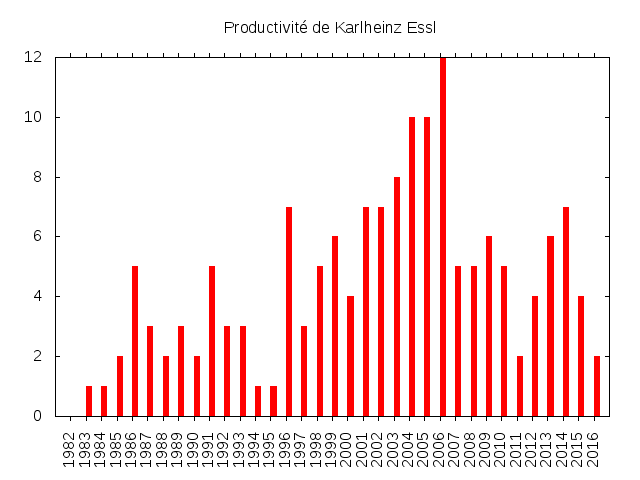
\includegraphics[width=12cm]{../Divers/plots/NumberOfWorks.png}
\caption{!!!}
\end{center}
\label{productivite}
\end{figure}

Ces œuvres d'une forme inédite sont le volet pratique du développement d'Essl, qui formule aussi de nouvelles notions sur le plan théorique, le conduisant à son rapport actuel à la musique algorithmique. Il élabore en particulier deux notions étroitement liées : celle de \guill{composition en temps réel} (\emph{Echtzeit Komposition}) et celle de \guill{???} \emph{Strukturgenerator}. \\
Voici, pour les appréhender, deux définitions qu'Essl donne aujourd'hui des algorithmes : \guill{[Les algorithmes] sont le fondement de ma pensée musicale, qui consiste à ne pas voir la musique seulement comme une expérience sensible, mais comme quelque chose qui comporte une multitude de structures plus profondes que l'on peut exprimer sous forme de modèles.}\footnote{\zitat{\dots~weil wir ja immer noch über Algorithmen sprechen. Dieser Begriff hat nichts mit Rhythmen zu tun, sondern ist nach diesem Mathematiker al-Chwarizmi benannt, der verschiedene mathematische Konzepte eingeführt hat. Diese sind auch die Grundlage meines Musikdenkens, Musik nicht nur als ein sinnliches Erlebnis zu sehen, sondern als etwas, das viele Tiefendimensionen hat, die sich in Form von Modellen ausdrücken lassen.}
{OMNIA IN OMNIBUS: Behind the Scenes - Karlheinz Essl im Gespräch mit Katharina Hötzenecker}}, et : \guill{Il y a la définition classique, qui provient plutôt des sciences de l'ingénieur, selon laquelle un algorithme est une sorte de recette de cuisine pour résoudre rapidement un problème. C'est une approche possible, mais il y en a une autre que je trouve plus intéressante. Elle consiste à envisager l'algorithme comme la définition d'un méta-modèle, duquel on peut obtenir différents résultats en modifiant les paramètres du système. C'est en ce sens que j'utilise le terme d'algorithme, et c'est ainsi que je le comprends dans les travaux de Gottfried Michael Koenig et Karlheinz Stockhausen.}.\footnote{\zitat{Man sollte sich zunächst die Frage stellen, was denn ein Algorithmus ist. Da gibt es klassische Definitionen, die eher aus den Ingenieurswissenschaften kommen, die beschreiben den Algorithmus als eine Art Kochrezept um schnell zu einer Lösung zu kommen. Dies ist ein möglicher Ansatz, aber es gibt noch einen weiteren, den ich interessanter finde. Dort begreift man einen Algorithmus mehr als Definition eines Metamodells, aus dem heraus durch Veränderung der Systemparameter verschiedenste Resultate entstehen. Diesen Algorithmusbegriff verwende ich selber und finde ihn auch in Werken und Arbeiten von Gottfried Michael Koenig und Karlheinz Stockhausen.}
{Intuition, Automation, Entscheidung. Der Komponist im Prozess algorithmischer Komposition}}. \\
Essl fait aussi plusieurs fois référence à la notion d'\emph{Urpflanze} de Goethe, une plante originaire imaginaire dont on pourrait dériver toutes les espèces plantes\footnote{\cite{goethe1993italienische}}. Le mot de \emph{modèle} est crucial dans l'idée de \emph{Strukturgenerator}\footnote{\cite{Strukturgeneratoren - Algorithmische Komposition in Echtzeit}}. Le produit des algorithmes que conçoit Essl possèdent une structure imposée commune, mais varient selon les paramètres fournis en entrée et le hasard\footnote{Le rôle du hasard dans la composition en temps réel fait l'objet de la partie \ref{???}.} interne des opérations exécutées par ces algorithmes. Le module \emph{Triller} de la \emph{Lexikon-Sonate}, étudié dans la partie \ref{???}, est un exemple simple de \emph{Strukturgenerator}. Tout ce que produit ce programme a une \emph{structure} de trille : un ensemble de quelques notes répétées à grande vitesse ; mais les trilles générées par différentes utilisations \emph{varient} par le nombre de notes différentes jouées, leurs hauteurs, la vitesse, la durée de la trille\dots~L'idée de définir des éléments musicaux comme des représentants d'un ensemble des possibles gouverné par une structure, sous la forme d'un système de règles, n'est toutefois ni nouvelle ni originale. Les règles strictes gouvernant le contrepoint classique relèvent exactement de ce cas de figure ; la seule nouveauté dans les \emph{Strukturgeneratoren} d'Essl est qu'ils sont \emph{actifs}, l'ordinateur permettant de créer la musique à la demande une fois le système de règles explicité et traduit en code informatique. On retrouve des procédés similaires dans nombre de musiques algorithmiques où le temps réel n'est pas nécessaire, et beaucoup de domaines usent de tels schémas, par exemple dans les jeux vidéos où il est aujourd'hui monnaie courante de générer ainsi des \emph{terrains}. \\
En revanche, l'originalité d'Essl réside dans la manière d'utiliser ces \emph{Strukturgeneratoren} : ce qu'il nomme la \guill{composition en temps réel}. Celle-ci peut être décrite comme la conjugaison de la composition algorithmique avec le temps réel. Les pièces de l'œuvre d'Essl répondant à cette appellation peuvent être réparties entre deux catégories : les \emph{installations} et les \emph{méta-instruments}. Les installations sont des programmes qui génèrent de la musique sans intervention humaine, généralement utilisées dans un lieu précis comme à l'intérieur d'un musée. À la différence d'un simple enregistrement, le son diffusé par un programme de type installation est élaboré au fur et à mesure. Ses caractéristiques notables sont en particulier l'absence de répétition, mais aussi de début et de fin en tant que tels. Les \emph{méta-instruments} sont des programmes offrant une interaction limitée (avec un \emph{instrumentiste}), mais dont le produit est du même type que celui d'une installation ; c'est en quelque sorte une installation dont les interactive dont un petit nombre de paramètres internes peut être modifié en temps réel. Un instrument traditionnel comme le violon laisse une liberté à celui qui en joue (hauteur, durée, volume des notes\dots), mais impose aussi certains paramètres du son (timbre, ambitus, nombre de notes pouvant être jouées simultanément\dots). C'est ce qui justifie cette appellation de méta-instrument, la principale différence étant que les instruments traditionnels sont déterministes (le même geste produira systématiquement le même son) mais généralement pas les méta-instruments programmés par Essl. Comme nous le verrons par exemple à travers l'étude détaillée de la \emph{Lexikon-Sonate}, c'est en combinant et associant des \emph{Strukturegeneratoren} qu'Essl réalise de tels programmes.

La spécificité de la composition en temps réel réside dans cette rencontre à la fois de la composition algorithmique et du temps réel, et représente une rupture qualitative par rapport à l'une et à l'autre. En effet, l'utilisation d'algorithmes n'était auparavant possible qu'en amont du moment de réalisation de la pièce. Quant aux technologies en temps réel, celles qui existaient déjà en musique électronique ne pouvaient être utilisées qu'en tant qu'instruments, pour produire et transformer du son. Les œuvres créées avec les prototypes d'ordinateurs en temps réel s'inscrivaient dans cette continuité, en utilisant la puissance de calcul pour élaborer de nouvelles transformations du son (par exemple \emph{Répons} de Pierre Boulez ou \emph{Antara} de George Benjamin). Essl a été l'un des premiers à mettre ces machines à calculer au service d'algorithmes de composition, et sans doute celui qui a le plus approfondi cette notion. Par la suite, avec la démocratisation de l'informatique (tant matérielle que logicielle), les pratiques similaires se sont multipliées, avec par exemple l'apparition au début du \XXIe~siècle du \emph{live coding} (utilisation d'environnements de programmation interactifs pour \guill{improviser} des codes, écrivant ainsi devant une audience le code informatique générant la pièce entendue en même temps).

%\zitat{+ description du processus de composition} !!!
%{Composing in a Changing Society - How does a composition come into existence ?}

\subsection{Descente de la tour d'ivoire}
\label{liberte}

Le dernier événement décisif dans le parcours d'Essl a lieu en 1997, lorsqu'il est invité au festival de Salzbourg (\emph{Salzburger Festspiele}) et présenté parmi les \guill{compositeurs de la nouvelle génération}. Le festival de Salzbourg, dédié à l'opéra, au théâtre et à la musique classique, est un événement de premier plan. Il est de plus davantage tourné vers la musique historique (en particulier celle de Mozart, né à Salzbourg) que vers la création contemporaine ; l'invitation fête à Essl marque donc un sommet de sa notoriété de compositeur.

Cet aboutissement est cependant un coup d'arrêt pour Essl. Il décide alors de changer radicalement sa posture de compositeur, en quittant la \guill{tour d'ivoire} dans laquelle il travaillait jusqu'alors. Au lieu de seulement composer seul des morceaux (ou des programmes) et d'en confier l'exécution à des interprètes (ou des machines), il souhaite s'ouvrir. Cela le conduit d'une part à devenir \emph{compositeur-performeur}, d'autre part à chercher à collaborer avec d'autres artistes pour ses créations futures.

Pour être à nouveau confronté au public, Essl devient donc \guill{\emph{performeur}}. La performance est une pratique artistique présente dans toutes les disciplines de l'art contemporain, supposant des actions éphémères à caractère unique\footnote{Au sens large, la musique générée par les programmes de composition en temps réel aurait donc un aspect performatif, au même titre que tout art de l'improvisation ; ce goût pour l'éphémère fait sans doute partie des motivations d'Essl à se tourner vers cette pratique et à la désigner ainsi.}, dont par exemple John Cage ou Yoko Ono font partie des initiateurs. La désignation est cependant exagérée : les \guill{performances} d'Essl sont avant tout des improvisations. L'improvisation fait partie des terrains de jeu privilégiés de la création musicale contemporaine, comme en témoigne par exemple le compositeur américain George Lewis : \guill{[L'improvisation] se porte bien un peu partout. Beaucoup de monde essaie d'apprendre à improviser, parce que cela a toujours été un moyen formidable pour découvrir comment faire de la musique. Il y a une ébullition très intéressante parmi les improvisateurs --- de nouvelles manières de structurer, des idées élaborées pour intégrer des partitions à l'intérieur de l'improvisation, de nouveaux sons, un élargissement des notions d'\emph{instrument}, de \emph{virtuose}, et du rôle du performeur.}
\footnote{\zitat{I think it [improvisation] is a healthy situation overall. Many people are trying to learn to improvise, because it has traditionally been a wonderful way to learn about the possibilities of making music. There is a lot of interesting activity among improvisers --- new methods of structuring, advanced ideas of how to integrate scores with improvisation, interesting new souunds, extended notions of what an \emph{instrument} is, what a \emph{virtuoso} is, what a performer's role is.}
{George Lewis in Composers and the computer, p. 81}}.

La volonté d'Essl de jouer devant un public comme il l'avait fait avec les groupes de rock de sa jeunesse se heurte toutefois à un problème majeur : il n'a aucun instrument dont il pourrait jouer. Bien qu'il ait comme nous l'avons vu joué du piano, de la guitare électrique et de la contrebasse, il n'a en 1997 plus aucune pratique instrumentale de haut niveau. Là encore, il trouve la solution en capitalisant sur son savoir-faire informatique : \guill{Il serait difficile d'imaginer mon travail sans les ordinateurs, même lorsque je fais de la musique instrumentale ; c'est grâce à l'ordinateur que j'ai pu quitter ma tour d'ivoire}
\footnote{\zitat{Ohne Computer wäre meine Arbeit schwer vorstellbar, selbst wenn ich Instrumentalmusik mache; dadurch war es mir möglich, aus meinem kompositorischen Elfenbeinturm auszubrechen.}
{Elektronische Musik / Komposition / Improvisation - Karlheinz Essl im Gespräch mit Silvia Pagano}}. Essl conçoit ainsi son propre \guill{instrument}, qu'il nomme \maze~(\emph{Modular Algorithmic Zound Environment}). Programmer son propre instrument est une pratique commune dans la musique contemporaine, ainsi témoigne le compositeur américain Curtis Roads : \guill{Beaucoup d'instruments digitaux peuvent être associés aux micro-ordinateurs de faible coût. La prolifération d'ordinateurs bon marché donne accès aux instruments intelligents à virtuellement n'importe quel musicien qui les souhaite.}\footnote{\zitat{Many digital instruments can be attached to inexpensive personal computers. The proliferation of inexpensive computers puts the capability of intelligent instruments within the reach of virtually every musician who wants them.}
{Composers and the computer, p. xvii}}.

\begin{figure}[h!]
\begin{center}
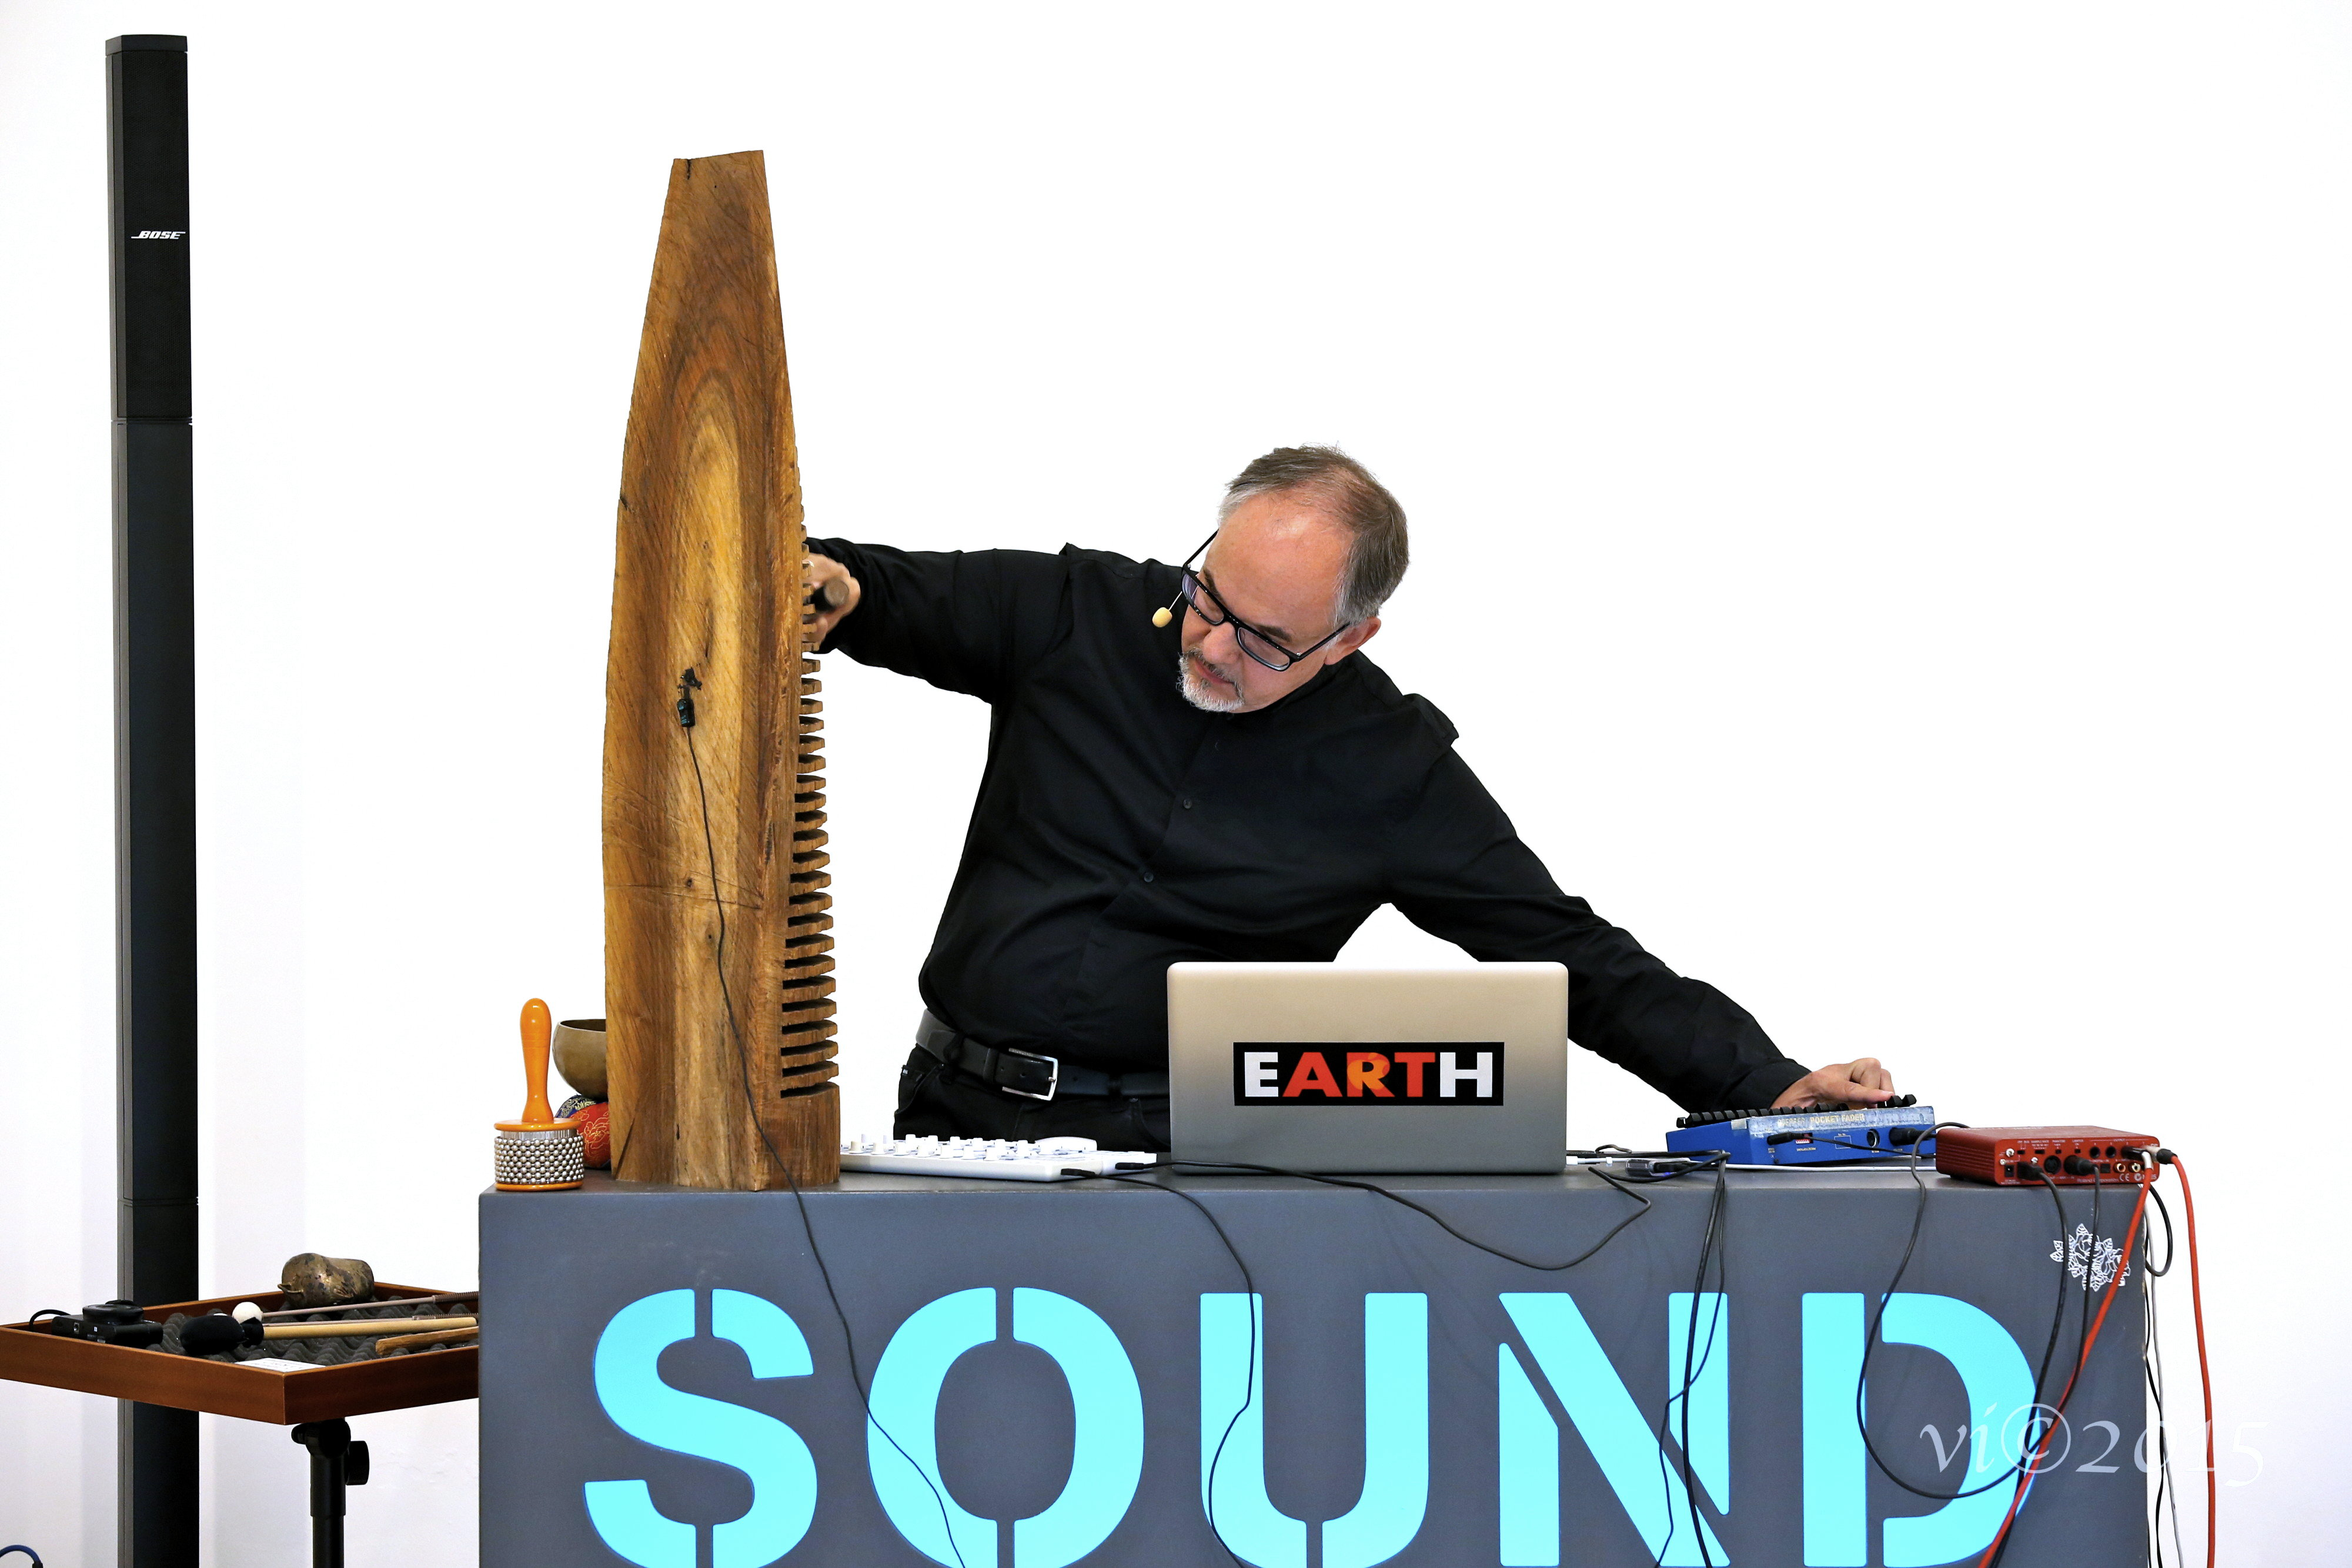
\includegraphics[width=10cm]{images/performance.jpg}
\caption{Karlheinz Essl réalisant une performance avec \maze --- Photo \copyright~Viktor Br\'azdil}
\label{performancephoto}
\end{center}
\end{figure}

Comme on peut le voir sur la photo \ref{performancephoto}, \maze~combine à la fois du matériel de musique électronique (pédales, micros, console MIDI\dots) et une interface logicielle (visible sur la photo \ref{mazephoto}) qui incorpore des algorithmes de traitement du son et des \emph{Strukturgeneratoren} pour la composition en temps réel. Les deux aspects, traitement du son et composition algorithmiques, sont présents simultanément. Là encore, Essl réalise une synthèse dans une opposition classique décrite par exemple dans !!! : \guill{[Tristan] Perich me dit que ses compositions émergent de l'improvisation, !!! --- en général le piano, qui est son instrument de prédilection. Il oppose ceci à d'autres compositeurs qui utilisent des algorithmes, ce qui entraîne des complications. \guill{Il y a une différence entre un processus qui fait partie de l'inspiration ou de votre ensemble d'outils, et un processus qui fait office de déterminant.}!!! Il préfère le premier.}\footnote{\zitat{[Tristan] Perich tells me that his compositions spring from improvisation, the mind at play --- usually at the piano, which is his main instrument. He constrats this with other composers who use algorithms, which introduce complications. \guill{There's a difference between process being part of the inspiration or the tool set that you have, and process being a determinant.} He prefers the former.}
{Composers and the computer, p. 264}}
Le \maze~est donc un méta-instrument dans le sens employé ci-dessus, et même un \guill{super-instrument}. Essl l'a en effet constamment développé et amélioré depuis sa création en 1998. On voit aussi sur la photo \ref{performancephoto} qu'il s'en sert pour augmenter\footnote{On parle en général d'\emph{instrument augmenté} lorsqu'un musicien ajoute des fonctionnalités électroniques à son propre instrument --- la guitare électrique est un instrument augmenté.} des instruments traditionnels.

\begin{figure}[h!]
\begin{center}
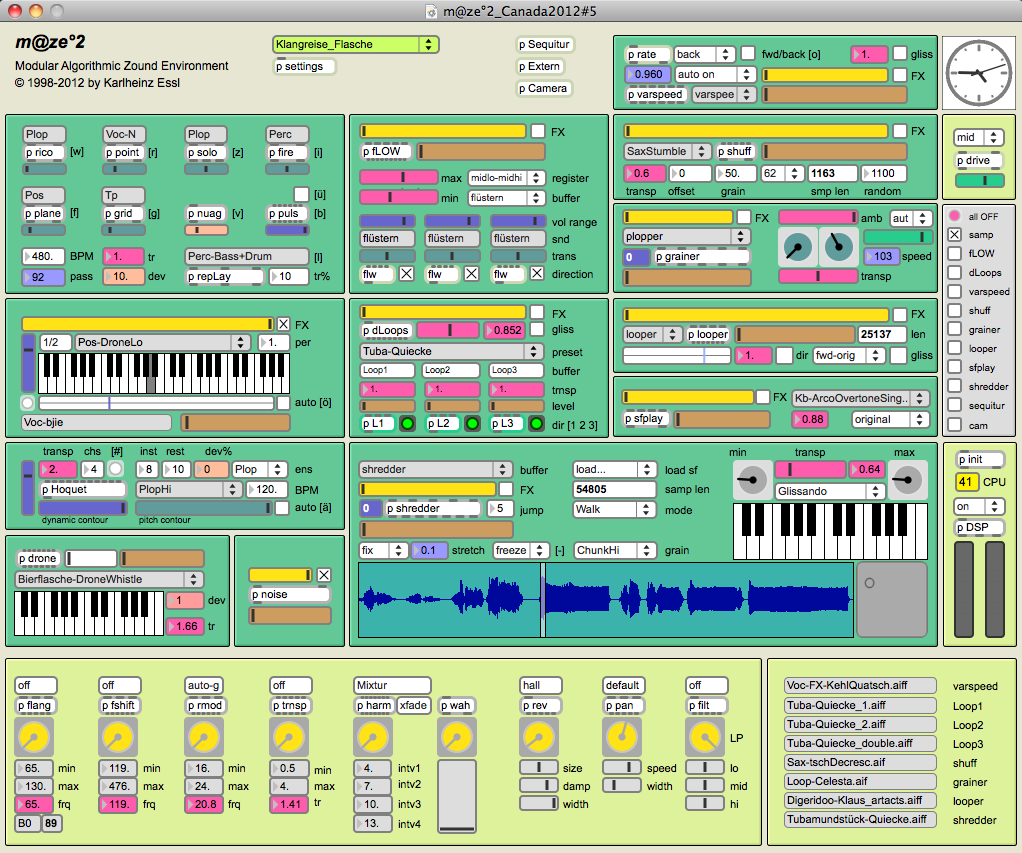
\includegraphics[width=8cm]{images/maze.png}
\caption{L'interface graphique du logiciel \maze --- Photo \copyright~Karlheinz Essl}
\label{mazephoto}
\end{center}
\end{figure}

L'ouverture voulue par Essl passe aussi par la collaboration avec d'autres artistes, musiciens (instrumentistes et compositeurs) ou non. Cela l'amène à composer de nouvelles formes et pour de nouveaux cadres, comme l'écrit Julieanne Klein : \guill{La production musicale d'Essl couvre tous les media possibles : orchestre, musique de chambre, théâtre musical, performance, musique électronique \emph{live}, musique informatique et électronique, méta-compositions et compositions en temps réel, méta-instruments, installations et paysages sonores, musique de film, visuels, compositions textuelles et pièces pour instruments solo. Cherchant constamment à étendre sa production créative, Essl collabore fréquemment avec des artistes d'autres disciplines, y compris des chorégraphes, des danceurs, des plasticiens, des vidéastes, des architectes, des poètes, des écrivains, et des graffeurs.}.
\footnote{\zitat{Essl's compositional output spans every possible medium: orchestral, chamber, musical theater/performance, live electronics, electronic computer music, real-time and meta compositions, meta-instruments, installations and soundscapes, film music, visuals, text compositions and works for solo instruments. Always looking to expand his creative output, Essl frequently collaborates with artists from other fields, including choreographers, dancers, visual artists, video artists, architects, poets, authors, and graffiti artists.}
{Julieanne Klein - A Portrait of the Composer Karlheinz Essl}	}

La concrétisation de cette nouvelle volonté d'ouverture passe par un projet d'envergure intitulé \emph{fLOW}. Il s'agit d'une entreprise polymorphe autour d'un programme homonyme générant un paysage sonore ; elle donne lieu à dix installations et vingt-deux performances (principalement en 1999 et 2000, mais les dernières ont lieu en 2007). Toutes incorporent le \maze, et chaque performance fait appel à des improvisateurs différents, jouant des instruments variés et issus de traditions musicales diverses (Nouvelle Musique, jazz expérimentale, improvisation livre, musique électronique).

Enfin, un autre événement important se produit en 1999 : l'ouverture du Essl Museum. Elle apporte deux explications supplémentaires à la nouvelle orientation de la carrière d'Essl. D'abord, elle s'inscrit dans la même ligne idéologique : Karlheinz Essl senior a fait construire ce musée pour mettre sa collection personnelle d'art contemporain à la disposition du public\footnote{La motivation de ce projet n'est peut-être pas seulement philanthropique --- sa vocation pourrait par exemple aussi être une entreprise de communication --- ; elle n'est du moins certainement pas économique, la construction du musée par l'architecte Heinz Tesar et son entretien étant assurés par le patrimoine de la famille Essl, sans aide publique. La mise à mal de ce patrimoine par la crise financière de 2007 à même conduit à un changement d'actionnaire majoritaire et à la décision de fermer le musée.}. Sur le plan matériel, elle offre une plus grande autonomie à Karlheinz Essl junior. Celui-ci dispose en effet d'un studio à l'intérieur du bâtiment, et d'un poste de conservateur chargé de la programmation musicale, grâce auquel il peut mettre ses productions en scène à l'intérieur des expositions, et nouer des relations en organisant des concerts.

\subsection{Essl et la culture numérique}

AUCTARIALITÉ

+ IL EST PROF IL TRANSMET

\subsection{Conclusion}

=> CLASSIQUE DE SA GÉNÉRATION

\zitat{... with complete autonomy since without public funding
... the famous names of 20th-century music with a clear inclination towards the composers that happily pursued the spirit of modernism even through the post-modern era. Hardly a coincidence, since kHz considers himself as belonging to that ilk.}
{An Extended Composer’s Desk - Composer Karlheinz Essl as the music curator of the Essl Museum}



\section{La composition en temps réel à travers ses programmes}

\subsection{Introduction}

Cette partie se propose d'analyser l'œuvre d'Essl à partir du code même de ses programmes. 
étudier la notion de \guill{composition en temps réel} dans l'œuvre d'Essl, !!! !!!

\subsection{La \emph{Realtime Composition Library}}

La \emph{Realtime Composition Library} (\emph{RTC-lib}) est une bibliothèque, c'est-à-dire un ensemble de fonctions réutilisables dans des programmes, développée par Karlheinz Essl dans le langage MAX/MSP. Son développement commence dès 1992, c'est-à-dire dès le moment où Essl a été mis en contact avec ce langage développé un an plus tôt par Miller Puckette (!!!), lors de son stage à l'IRCAM. Son origine remonte même à 1988, si l'on considère qu'Essl a commencé par implémenter dans ce nouveau langage les algorithmes de composition qu'il avait déjà développés en xLOGO, rassemblés dans une bibliothèque intitulée \emph{COMPOSE}.

Cette bibliothèque est le socle de la plupart des œuvres réalisées par Essl impliquant la programmation. Il en recense 56 à ce jour : partitions, programmes, installations \emph{works-in-progress}\dots, parmi lesquels certaines de ses créations majeures comme les \emph{Sequitur}, \emph{fLOW} (!!!) ou encore la \emph{Lexikon-Sonate}, que !!!. C'est aussi à partir d'elle qu'il a conçu l'\guill{instrument} qu'il utilise lors de ses performances, le \maze. Elle est distribuée sous licence libre. Elle est disponible en téléchargement et il est possible de l'utiliser et de la modifier gratuitement, à la seule condition d'en citer les auteurs.

Dans ce qui suit, je propose une description détaillée et une analyse de cette bibliothèque, en commençant par !!!


\subsubsection{Description}

MAX/MSP est un \emph{langage de programmation graphique}, c'est-à-dire un langage de programmation dans lequel les programmes ne sont pas écrits en texte mais construits à partir d'éléments graphiques. Dans le cas de MAX, ces éléments sont des boîtes ou \guill{\emph{patches}} possédant des entrées et des sorties, et des liens qui permettent à ses fonctions d'interagir --- typiquement : relier une sortie d'un \emph{patch} à l'entrée d'un autre. Un exemple (figure !!!). Il existe deux modes d'édition distincts, l'un pour construire le \guill{circuit} du programme, l'autre permettant de l'exécuter et de modifier les paramètres (valeurs numériques, impulsions ou \guill{\emph{bangs}}, curseurs etc.). MAX ayant été développé expressément pour la musique assistée par ordinateur, il contient de nombreux objets dédiés comme des entrées et sorties MIDI, ou dédiés au traitement du son\footnote{En réalité, MAX ne permettait à l'origine que la manipulation de données au format MIDI ; c'est la bibliothèque MSP, ajoutée en 1997, qui permet le traitement de signal audio (\emph{Digital Signal Processing, ou DSP}). Une autre bibliothèque d'importance nommée Jitter a été ajoutée en 2002, qui permet synthèse la manipulation graphiques.}.

\begin{figure}[h!]
\centering
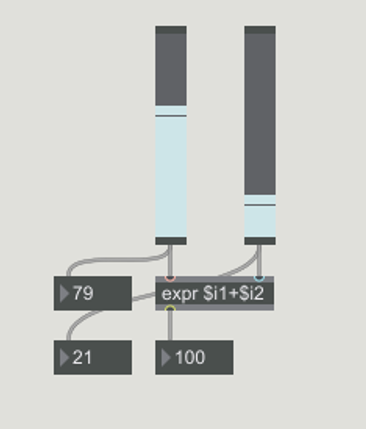
\includegraphics[width=5.5cm]{images/MAXbase.png}
\label{maxmsp}
\caption{Un programme basique en MAX/MSP : l'affichage et l'addition de deux entiers déterminés par des \emph{sliders}.}
\end{figure}


La \emph{RTC-lib} est divisée en huit rubriques, qu'illustre en outre un tutoriel (voir figure !!!). Les trois premières rubriques, \emph{Toolbox}, \emph{Chance} et \emph{Lists}, contiennent des objets « basiques ». Les trois suivantes, \emph{Harmony}, \emph{Rhythm} et \emph{Envelopes}, des objets « de composition », et les deux dernières, \emph{MSP} et \emph{Jitter}, regroupent les fonctions directement liées aux sorties son et vidéo. À ce jour il y a en tout 177 objets. 140 sont écrits par Essl, les autres en collaboration avec ou d'après d'autres compositeurs ou chercheurs\footnote{R. Albert Falesch, Charles Baker, Frank Barknecht, John Chowing, Chris Dobrian, Richard Dudas, Gerhard Eckel, Peter Elsea, Philippe Gruchet, Gary Lee Nelson, Serge Lemouton, James McCartney, Iain Mott, Eric Singer, Les Stuck et David Zicarelli.}.



On y trouve de nombreuses fonctions très simples, en particulier dans la rubrique \emph{Toolbox} : calcul de l'inverse, de l'opposé, accumulateur\dots~D'autres corrigent ou améliorent des fonctions pré-existantes, comme la division euclidienne (ne fonctionnant à l'origine qu'avec un numérateur positif) ou l'arrondi (rendu paramétrable par Essl). \\
C'est aussi le cas de la rubrique \emph{Lists}, dont la plupart des fonctions proposent simplement une forme plus ergonomique de fonctions pré-existantes, parfois simplement en leur donnant un nom plus clair. Elle contient ainsi des fonctions calculant la longueur d'une liste, l'intersection de deux listes, scindant une liste\dots~On en trouve d'autres qui résument en une seule fonction des opérations très simples mais utiles et donc amenées à être utilisées souvent. Par exemple la fonction \emph{butfirst} (respectivement \emph{butlast}) cache simplement, en lui donnant une signification explicite, la scission d'une liste après son premier (respectivement avant son dernier) élément. \\
Enfin, les dernières fonctions avant tout pratiques que contient la \emph{RTC-lib} sont des conversions présentes dans chaque rubrique. Elles permettent au compositeur de manipuler les différents outils de la bibliothèque sans se soucier de leur compatibilité de type, qui peut être immédiatement gérée par ces convertisseurs. Cela va de transformations de pitch en note MIDI ou en fréquence à celles entre différentes sorties sons, ou encore à celles entre durées relatives et absolues.

\subsubsection{Analyse}

\paragraph{Théorique}

\paragraph{Technique}

\paragraph{Esthétique}

Le cœur de la partie véritablement compositionnelle de la \emph{RTC-lib} réside à mon sens dans la rubrique \emph{Chance}. En effet, bien qu'elle contienne comme \emph{Toolbox}, \emph{Lists}, \emph{MSP} et \emph{Jitter} des outils basiques représentant des fonctions simples, c'est la variété des générateurs aléatoires présents dans celle-ci qui rend possible la liberté de développer des algorithmes musicaux. Et c'est pour beaucoup à partir de cette variété que se construisent les fonctions des modules \emph{Harmony}, \emph{Rhythm} et \emph{Envelopes}. Là encore, l'ergonomie est une préoccupation importante ; tous les générateurs sont ainsi déclinés en deux fonctions, selon qu'ils fournissent leurs résultats séquentiellement, ou directement sous la forme d'une liste. Là encore, toutes les fonctions ont un code relativement simple, parfois largement fondé sur des fonctions standard de MAX, comme la génération sérielle présente nativement dans la fonction \emph{xrandom} rebaptisée \emph{series}. \\
On retrouve la plupart des générateurs aléatoires classiques : probabilité uniforme, sérialisme, chaînes de Markov, mouvement brownien. Certains sont déclinés en plusieurs variantes intégrant des paramètres supplémentaires (pondérations, interdiction de répétitions...). On remarque la présence moins commune de plusieurs générateurs reposant sur des échelles logarithmiques, mais l'absence de générateurs reposant sur des distributions de probabilité comme les lois de Gauss ou de Poisson. D'une manière générale, on trouve presque exclusivement - c'est-à-dire à l'exception du générateur de mouvement brownien, \emph{brownian} - des générateurs discrets et non continus.

Si l'on se penche maintenant sur les rubriques dites « de composition », on peut y distinguer trois sortes de fonctions. \\
D'abord, il y a les fonctions spécifiques aux données du son concernées, qui implémentent des comportements et des outils classiques. Par exemple, la fonction \emph{neutral-harmony(n,i)} génère séquentiellement des notes à partir de n par déplacement d'un intervalle i puis de son complémentaire, tandis que la \emph{metro-dev\%} modélise un instrumentiste humain en introduisant des approximations dans un battement parfaitement régulier, et que la fonction \emph{panning} calcule la distribution stéréo des volumes pour simuler le déplacement de la source sonore. Parmi cette première sorte, toute une sous-section de \emph{Harmony} est dédiée aux manipulations dodécaphoniques usuelles. \\
La deuxième sorte de fonctions est une application des différents générateurs aléatoires et de certaines opérations de listes à chaque rubrique. Concrètement, ce sont à peu de choses près des convertisseurs qui transforment les résultats de ces générateurs en données représentant des hauteurs de notes (entiers d'un certain ensemble), des rythmes (\emph{bangs} émis, ou entiers correspondant à des ?????????????ED), et des vélocités (entiers entre 0 et 127). Néanmoins cette description est un peu réductrice, en ce que ces fonctions considérées de l'extérieur dépassent la simple conversion de données, possèdent un véritable contenu sémantique.
Les fonctions de la troisième sorte regroupent les précédentes. Elles possèdent de nombreux paramètres d'entrée, dont la possibilité de choisir parmi les différentes méthodes aléatoires utilisables. C'est typiquement le cas du très complet \emph{super-rythm}.

J'ai écrit que la plupart des algorithmes présents dans cette bibliothèque était plutôt simples ; en terme de complexité algorithmique, ils sont tous au plus linéaires (ce qui est, effectivement, une complexité faible). Cette complexité n'est en outre jamais apparente dans les algorithmes d'Essl (sous forme par exemple de boucles ou, plus évident en MAX, de récursivité), mais seulement dans les sous-procédures élémentaires qu'il appelle, plus précisément les manipulations de listes et les objets de type \emph{métronome}. \\ 
%[Ici aussi il aurait fallu quelques précisions sur la complexité algorithmique. J'ai supposé que vous étiez familier avec cette notion, primordiale pour tout informaticien théorique, mais j'ai l'impression qu'il y a assez peu de porosité et qu'elle est peu ou mal connue par ailleurs.]

S'il fallait décrire un « style » de programmation dans la \emph{RTC-lib}, je dirais que c'est une pensée avant tout fonctionnelle. Cela signifie que le paradigme avec lequel Essl approche la programmation lui fait voir les algorithmes comme des fonctions qui \emph{calculent} (pensée fonctionnelle) plutôt que par exemple comme des listes d'instructions à exécuter (pensée impérative). Une illustration simple en serait la fonction \emph{remove} de la rubrique \emph{Lists} : pour supprimer le \emph{n}-ième élément d'une liste \emph{L}, Essl calcule les sous-listes \emph{L1} et \emph{L2} séparées au niveau de cet élément, puis la liste \emph{L1'} comme \emph{L1} privée de son dernier élément, et enfin le résultat comme la jonction de \emph{L1'} et\emph{L2}. Une pensée impérative aurait plutôt fait reculer d'un rang chaque élément à partir du \emph{n+1}-ième. Cela n'a rien de surprenant car c'est la manière de programmer naturellement induite par le langage MAX, et associée avec l'utilisation de listes, omniprésentes dans la \emph{RTC-lib} (la structure de données équivalente de la programmation impérative étant le tableau). Il est cependant intéressant de noter qu'Essl, qui a commencé à programmer avec des langages impératifs (Basic, LOGO) maîtrise parfaitement les codes du paradigme de programmation le mieux adapté dans ce contexte - malgré l'absence de récursivité, autre caractéristique essentielle de la pensée fonctionnelle. D'une manière générale, lesl algorithmes sont codés de manière directe, concise, et très claire. On peut même remarquer parfois le choix, augmentant cette concision, d'étapes \emph{hard-coded} : au lieu de faire calculer une sous-fonction de manière procédurielle, l'ensemble de ses valeurs est intégralement décrit en donnée.

Enfin, quelques remarques sur les choix esthétiques sous-jacents. L'influence de l'école sérielle est très présente, ainsi que celles de Gottfried Michael Koenig et de Karlheinz Stockhausen, à qui plusieurs algorithmes font des emprunts (ils sont nommés dans les descriptions). La pensée est aussi très « pianistique » dans le sens où les notes sont décrites par d'uniques hauteur et vélocité (comme sur un piano mais pas sur un violon, où le son d'une même note peut évoluer dans le temps). Il aurait pu en être autrement compte tenu de l'intérêt qu'Essl accorde au son en général, mais cela n'a rien d'étonnant dans un langage de programmation qui privilégie la notation MIDI, et un langage musical marqué par la pensée sérielle. Rythmiquement, on peut noter un affranchissement de la notation sur partition car ce ne sont jamais des noires, croches, doubles, etc., qui sont manipulées, mais exclusivement des durées absolues. Enfin, lorsqu'il s'agit de générer les ensemble de valeurs parmi lesquelles opérer des choix aléatoires, Essl a une préférence nette pour les échelles logarithmiques - sans doute parce qu'elles permettent à la fois précision et contrastes -, disponibles presque systématiquement.

En conclusion, il apparaît que les moyens techniques nécessaires à l'utilisation de cette bibliothèque en temps réel concernent avant tout l'interaction entre l'unité de calcul et les périphériques de son ou d'image. Les algorithmes utilisés par Essl sont d'une complexité très en-deçà non seulement des capacités non seulement des processeurs actuels, mais aussi de leurs prédécesseurs. [Il faudrait que je creuse pour avoir une idée de ce qu'on peut exécuter en temps perçu comme réel sur les \emph{personal computers} des trente dernières années, mais je soupçonne que c'était déjà le cas, ou alors presque, en 1991.] Il possède une bonne maîtrise technique, à la fois dans l'efficacité des algorithmes et dans la manière de les présenter et documenter (sans quoi l'entretien du code et son utilisation par d'autres serait beaucoup moins aisée). Mais c'est son savoir-faire de compositeur qui ressort, qui se reflète dans le choix des algorithmes plutôt que dans leur implémentation. Bien que ceux-ci soient « simples » au sens informatique, la \emph{RTC-lib} est très complète car d'une part chaque algorithme de composition peut produire des résultats très divers selon la leur paramétrage, et ils sont facilement combinables, pour créer des générateurs de musique dont les modules de la \emph{Lexikon-Sonate} sont d'éloquentes illustrations.



\subsection{Analyse}



% D'après http://doornbusch.net/ !!!
% https://en.wikipedia.org/wiki/Instructions_per_second#MIPS !!!
\begin{figure}
\begin{center}
\begin{tabular}{|c|c|c|c|}
\hline
\textbf{Année} & \textbf{Mips} (!!!) & \textbf{Modèle} & \textbf{Type} (!!!) \\
\hline
1954 & 0,000640 & IBM 704 & Mainframes \\
\hline
1969 & 3,3 & IBM 360/85 & Mainframes \\
\hline
1973 & 0,065500 & DEC PDP 11/45 & Mini \\
\hline
1977 & 0,230 & Apple II & Micro \\
\hline
\textbf{1982} & \textbf{2,188} & \textbf{Atari ST} & \textbf{Mini} \\
\hline
1985 & 1,6 & VAX 11/785 & Mini \\
\hline
\textbf{1998} & \textbf{525} & \textbf{iMac G3} & \textbf{Micro} \\
\hline
2003 & 3100 & iMac G5 & Micro \\
\hline
2008 & 50000 & Apple Mac Pro & Micro \\
\hline
\end{tabular}
\end{center}
\caption{Tableau MIPS !!!}
\label{tableaumips}
\end{figure}

% « Many functions that are often useful in algorithmic composition are provided with this library - therefore the composer could concentrate rather on the composition than the programming aspects. » Il s'agit effectivement principalement de fonctions assez simples techniquement, mais conçues de manière très ergonomique.

\zitat{Most of these objects are geared towards straightforward processing of data. By using these specialized objects together in a patch, programming becomes much more clear and easy. Many functions that are often useful in algorithmic composition are provided with this library - therefore the composer could concentrate rather on the composition than the programming aspects.}
{RTC-lib}

\subsection{Quelle \guill{composition en temps réel} ?}

diese Ircam Signal Processing Workstation entwickelt. Das war ein NeXT Computer mit einer speziellen Soundkarte, mit einem ganz tollen Prozessor, der konnte in Echtzeit Klangsynthese und Klangmanipulationen, Soundprocessing machen

\zitat{It is interesting to note that we have with Cage two ways of using randomness for music composition. One, inhreited from Duchamp, is what can be called \emph{internal chance}: randomness is used at composition time to determine the score, which is then written and closed. The other can be called \emph{external chance}: the score is open to real-time chance operation and external perturbation. In that respect, \emph{4'33''} is certainly the best and minimal example of external chance.}
{Philippe Codognet, New computational paradigms for computer music, p. 160}
=> Ça se rejoint dans RTC !!!

\zitat{Mais le temps réel est une notion technologique avant d'être une notion musicale. C'est en fait une illusion. Le temps réel n'existe jamais dans la réalité technologique parce qu'une machine met toujours un certain temps, même si celui-ci est extrêmement bref, pour effectuer ses calculs.}
{La musique du temps réel, p. 41}

\zitat{En musique, on parle de temps réel à partir du moment où le laps de temps entre le début du calcul et la livraison du résultat d'une opération informatique est suffisamment bref pour ne pas être perçu.}
{La musique du temps réel, p. 42}

\zitat{Le grand avantage du temps réel, ce n'est pas un gain de temps pour le compositeur --- au contraire cela représente une difficulté supplémentaire à maîtriser --- mais c'est qu'il intègre l'interprétation dans la musique électronique ; auparavant ces deux domaines restaient étrangers l'un à l'autre.}
{La musique du temps réel, p. 44-45}

\zitat{Weil man sich beim Improvisieren nicht (wie beim Komponieren) "out of time" befindet, sondern mitten im Zeitablauf steckt, entstehen aus dieser Verantwortung und aus diesem Zwang heraus Situationen, die man als Komponist am Schreibtisch nicht planen kann.}
{Improvisation über "Improvisation" - Karlheinz Essl \& Jack Hauser}

\zitat{My formal thinking takes place in a bipolar field of tension, namely that between work and process. (…) For me, the most captivating aspect of composing is the reconciliation of these opposites, though each time in a different way.}
{Composing in a Changing Society - How does a composition come into existence ?}

\zitat{I immediately felt in love with it for it offered the possibility of realtime processing and interactivity. (In LOGO, it took many hours to calculate a score list which I had to transcribe into of musical notation in order to analyze it - a very time-consuming procedure).}
{RTC-lib}

\subsection{La \emph{Lexikon-Sonate}}

\zitat{\dots~l'œuvre qui nous est restituée chaque fois dans sa totalité, n'en reste pas moins chaque fois incomplète. Est-ce un hasard si tutelles poétiques sont contmeporaines de la loi physique de \emph{complémentarité}, selon laquelle on ne peut montrer simultanément les différents comportements d'une particule élémentaire et doit, pour les décrire, utiliser divers modèles qui \guill{sont justes lorsqu'on les utilise à bon escient, mais se contredisent entre eux et dont on dit, par suite, qu'ils sont réciproquement complémentaire} ? Ne peut-on dire pour ces œuvres d'art, comme fait le savant pour la situation expérimentale, que la connaissance incomplète d'un système est une composante essentielle de sa formulation ?}
{L'Œuvre ouverte, p. 30}

\zitat{Aujourd'hui, l'accent est mis sur le processus, sur la possibilité de saisir \emph{plusieurs ordres}. Dans la réception d'un message structuré de façon ouverte, l'\emph{attente} implique moins une \emph{prévision de l'attendu} qu'une \emph{attente de l'imprévu}.}
{L'Œuvre ouverte, p. 105}

\zitat{Contrainte par la logique de ses propres faits, la musique, en un mouvement critique, a dissous l'idée d'œuvre achevée et rompu avec le public. [\dots] Les seules œuvres qui comptent aujourd'hui sont celles qui ne sont plus des \guill{œuvres}.}
{Adorno, p. 41-42}

\zitat{I want to challenge the listener not just to consume the piece but by listening becoming something like a co-creator, being a partner of the composer and the composition itself.}
{Profile Karlheinz Essl - Karlheinz Essl in conversation with Joanna King}

\zitat{Die Lexikon-Sonate ist voll absurder Situationen; die isolierten Musiksprachfetzen aus der Geschichte der Klaviermusik werden in immer neuen ZUFALLSNACHBARSCHAFTEN zusammengesetzt; sie rufen Erinnerungen hervor, die aber aus dem Kontext gerissen und in eine irrationale Struktur eingebunden werden.}
{Irreal-Enzyklopädie - Bernhard Günther - Einer metaphorischen Reise zur Lexikon-Sonate von Karlheinz Essl}

\zitat{Einer der Ausgangspunkt ist meine Hassliebe zu diesem Instrument, dem Klavier. Ich wurde mit sieben Jahren gezwungen, Klavier zu lernen; ich wollte Blockflöte spielen. Trotzdem war ich am Klavier nie gut. Es war immer frustrierend, zu sehen, dass ich das, was ich im Kopf hatte, auf den Tasten nicht adäquat umsetzen konnte. Meine ersten Kompositionversuche waren natürlich trotzdem Klavierstücke, aber ich habe sonst kein einziges Klavierstück geschrieben bis jetzt, und ich kann mir auch nicht vorstellen, ein Klavierstück zu schreiben. Das einzige, was mir möglich war: Ein Klavierstück zu machen, das ganz absurde Kriterien erfüllt.}
{Der Wiener Komponist Karlheinz Essl (Hanno Ehrler)}

\zitat{Ein Computer wird nie müde. Mit dem Computer kann man eine Musik in Szene setzen, die nie aufhört, das geht mit Musikern natürlich nicht.}
{Elektronische Musik / Komposition / Improvisation - Karlheinz Essl im Gespräch mit Silvia Pagano}

\subsection{Conclusion : Essl et l'ordinateur}

\zitat{Essl nutzt die heutigen Möglichkeiten der TECHNIK als Mittel, musikalische Möglichkeitsstrukturen zu schaffen, die in der Lage sind, unbeliebig Anderes zu realisieren als die Vorstellung des Komponisten.}
{Irreal-Enzyklopädie - Bernhard Günther - Einer metaphorischen Reise zur Lexikon-Sonate von Karlheinz Essl}

\zitat{In meinem Aufsatz Computer Aided Composition, den ich 1991 veröffentlicht habe, geht es genau um die Frage, was der Computer dem Komponisten zurückgibt. Darin habe ich zwei Sachen postuliert. Erstens: Wir müssen den Computer selber programmieren, d. h. wir müssen unsere eigenen persönlichen individuellen kompositorischen Ideen und Fragestellungen in Form von Computerprogrammen formulieren. Zweitens: Der Computer wird dadurch zum Werkzeug, das diese Regelsysteme (die ja nicht bloß abstrakt sind, sondern von kompositorischen Ideen ausgehen) anwendet, dabei Ergebnisse erzeugt und uns diese dann widerspiegelt. In den vom Computer errechneten Resultaten erkennen wir die Tragweite unserer kompositorischen Ideen. Ich vergleiche den Computer (bzw. die Software, die auf ihm läuft) gerne mit einem Spiegel, der das, was wir uns vorstellen, sehr rasch realisieren kann.}
{Intuition, Automation, Entscheidung. Der Komponist im Prozess algorithmischer Komposition}

\section{Démocratisation ?}

\zitat{Le poète le plus ésotérique ou le théologien le plus abstrait sont beaucoup plus concernés que le scientifique par l'approbation des non-spécialistes, bien qu'ils puissent être encore moins concernés que lui par l'approbation en général.}
{Kuhn}

\zitat{À mesure que l'abstraction gagne, les frontières géographiques s'élargissent, la poésie n'a plus de pays, elle est prête pour le voyage dans l'universel.}
{Les théories de l'art, p. 25}

\zitat{L'invention du micro-ordinateur par les radicaux californiens, sur laquelle nous allons revenir, avait pour obkectif explicite de battre en vrèche la centralisation et la possession des précieuses \guill{informations} par quelques privilégiés. La \guill{guérilla} micro-informatique a en partie porté ses fruits. Elle a constitué une sorte de révolution dans la révolution et son radicalisme a été en grande partie à l'origine de la \guill{culture informatique}, partagée dans un large public et facteur de démocratisation de la vie sociale et du savoir.}
{Breton, intro chap 11}

\zitat{L'informatique de la deuxième période, qui avait été considérée comme une menace pour les libertés, a acquis avec le micro-ordinateur une image beaucoup plus \guill{conviviale}. Pour les générations nées dans les années soixante, informatique et liberté sont désormais synonymes. La société de l'information centralisée devient progressivement une société de communication, une société de réseaux.}
{Breton, p. 206}

\zitat{L'espace du réseau met en jeu un type de liaison multimodale entre les utilisateurs sans précédent : la liaison de \emph{tous vers tous}. Chaque internaute est à la fois récepteur et émetteur. Il peut recevoir des messages de n'importe quel(s) autre(s) émetteur(s) et, à son tour, lui (leur) adresser des messages, messages eux-mêmes mutlimodaux, composés de texxtes, d'images (fixees ou mobiles) et parfois de sons. Il s'agit d'un système de communication totalement différent des médias de masse (radio, cinéma, télévision), qui fonctionnent sur le type de liaison \emph{un vers tous}, où le retour immédiat et interactif de tous vers un n'est pas possible.}
{L'art numérique, p. 63}

\zitat{L'ambitieuse volonté d'une communication universelle est contrecarrée par la réalité. Le public attendu, innombrable, multi et transculturel, reste encore un public de spécialistes très liés au monde de l'art et très infentifiables socialement. Les \guill{communautés virtuelles} sont en fait des microcosmes assez fermés, avec déjà leurs traditions et leurs orthodoxies. De sorte qu'il est légitime de s'interroger sur les limites d'un art en réseaux et, au-delà, sur les limites du paradigme réticulaire aujourd'hui dominant, qu'on pourrait décrire comme un paradigme de l'\guill{horizontalité}.}
{L'art numérique, p. 79}

\zitat{L'Internet apparaît en tout cas comme le lieu de cette mémoire à venir, comme musée virtuel global. C'est à la fois un \emph{nouveau support}, qui étend considérablement les possibilités de diffusion et de conservation de la mémoire, et un \emph{nouvel enjeu} de la mémoire, un puissant vecteur de dynamisation du musée dans sa virtualisation, qui permettrait de compenser la muséification de certains de nos espaces physiques (urbains ou ruraux).}
{L'art numérique, p. 231}

\zitat{The development of these digital synthetisers is extremely promising. They help bring together the generality of digital sound synthetis with appealing real-time possibilities. Until recently, it was possible to use the computer for music only in large institutions. But powerful music systems may become available at low price, and this new economic situation will completely change the status of digital electronic music. Digital systems are becoming private tools for the independent composer.}
{???}

\zitat{Vom Bewohner eines Elfenbeinturmes bin ich peu-à-peu zum global citizen geworden, dessen Tätigkeit sich nicht mehr allein im Verfertigen komplexer Partituren erschöpft. Durch den Kontakt mit Gleichgesinnten, der zunächst hauptsächlich über Mailing-Lists ausgetragen wurde, reiften in mir neue Ideen, die den für mich bislang gültigen Werkcharakter von Musik immer fragwürdiger werden ließen.
Der nicht-hierarchische Charakter des Internets mit seiner rhizomatischen Struktur zeigt vielfache Entsprechungen zu meiner persönlichen Sichtweise, Musik als kommunikatives Netzwerk aufzufassen und dieses auch sinnlich erfahrbar zu machen.}
{net.music}

\zitat{Das sehe ich mittlerweile auch ganz deutlich bei eurem Performance-Projekt LUX FLUX. Das ist sehr offensichtlich und hat mich sehr beeindruckt. Für den Betrachter wird klar, das ihr mit einem Alphabet sprecht, das begreifbar ist.}
{Improvisation über "Improvisation" - Karlheinz Essl \& Jack Hauser}

\zitat{Thus only musicians may really experience the formal openness of a musical text since they are confronted with the alternatives and can take decisions while playing.}
{Technological Musical Artifacts (Gerhard Eckel)}

\zitat{+ analyse de la Homepage}
{Der Wiener Komponist Karlheinz Essl (Hanno Ehrler)}

\zitat{GF: Do you think that the net has a specific musical potential? KHE: From my personal experience, I think that the most important thing is the communication aspect.}
{NET Music - Karlheinz Essl talking to Golo Föllmer}

\zitat{Ich wollte ganz bewusst ein sehr knappes Material verwenden, das auch leicht wiedererkennbar ist. Diese Fanfare ist ja im Grunde ein in uns eingebranntes Zeichen, dass wir als Bestandteil unserer Kultur erkennen, weil man es schon so oft gehört hat. Man denke nur an den Film Apocalypse Now. Es gibt bestimmte signalhafte Musiken, wie auch die Fünfte Beethovens; dieses Kopfmotiv, das kennt man einfach. Das heißt, das braucht man nur anspielen und jeder weiß sofort, was das ist.}
{Wagner in Translation - Karlheinz Essl im Interview mit Annegret Huber}

\zitat{When not composing himself, he is busy inspiring a generation of younger composers in his position as Professor of Composition at the Vienna University of Music and Performing Arts. Beyond this, Essl is also influential in the cultivation and dissemination of new art, particularly seen in his co-direction of the family-run Essl Museum, a modern art museum based outside of Vienna. Here Essl has fueled a series of innovative programs that expand the boundaries of sonic landscape; educating audiences, inspiring young composers, and erasing the bourgeois line so often perceived in traditionally classical venues.}
{Julieanne Klein - A Portrait of the Composer Karlheinz Essl}

\zitat{Ich mache keine abstrakte Musik, die man nur versteht, wenn man eine spezielle Ausbildung hat, oder Wissen oder viel Erfahrung. Mir geht es vor allem um das Unmittelbare, das Ekstatische, das sich demjenigen erschließt, der bereit ist sich dem hinzugeben. Ich habe die Erfahrung gemacht, dass es nicht darauf ankommt, ob man seinen Schönberg oder Webern studiert hat, seinen Mozart oder Bach. Wenn man die Bereitschaft hat sich zu öffnen, dann kann man sehr viel erleben. Ich glaube, dass das Hören immer ein interaktiver Prozess ist, letztlich würde ich sogar sagen, dass die Musik im Hörer selbst entsteht - durch den Akt des Hörens.}
{Rückblick / Vorschau - Der Komponist Karlheinz Essl im Gespräch mit Annelies Kühnelt}

\zitat{Deshalb glaube ich, dass das Wissen darum für den Hörer nicht unbedingt nötig ist. Die Stücke sollten deshalb sinnlich, also ganz im Bereich des Klanglichen, rezipiert werden. In beiden Fällen gehe ich jedoch vom Hören aus: die Strukturgeneratoren (ob sie nun die Lexikon-Sonate, Amazing Maze oder Champ d'Action betreffen) gehen immer von Wahrnehmungsphänomenen aus, niemals von abstrakten oder gar mathematischen Prämissen. Deshalb meine ich auch, dass sich meine Musik am besten durch offenes, bereitwilliges und vorbehaltloses Hören erschließt, in einem aktiven Wahrnehmungsprozess, in dem sich der Hörer aufgrund seiner jeweiligen persönlichen Voraussetzungen sozusagen seine eigene Fassung der Komposition mitkomponiert. Hören wird hier nicht zum bloßen Abbilden und Entziffern einer vorgegebenen Wirklichkeit, sondern zu einer schöpferischen Konstruktion.}
{Karlheinz Essl / Bernhard Günther - Realtime Composition - Musik diesseits der Schrift}

\zitat{Du brauchst nur ein Websearch machen. Mittlerweile tauche ich auch immer wieder in Blogs auf: „Da gibt’s übrigens so einen verrückten Typen in Wien, der macht irre Sachen. Da gibt’s fLOW und den REplay PLAYer...“ oder sie sprechen von einer „eine schattenhafte Figur...“. Das kommt nicht unbedingt aus dem Bereich der Hochkultur, wie wenn man in der Carnegie Hall eine Aufführung hat. Aber es vermittelt einem das Gefühl, dass man irgendwie präsent ist. [...] Wohingegen die Sache mit Internet unheimlich schnell reagiert und sich besser verbreitet und nicht von wenigen Zentren aus gesteuert wird.}
{Elektronische Musik / Komposition / Improvisation - Karlheinz Essl im Gespräch mit Silvia Pagano}

\zitat{JF: Curtis Roads behauptet: „Some composers who use formal methods feel that what the listener hears is secondary. They take professional satisfaction in knowing that their structures are logically generated, whether or not they are perceived as such.” Welchen Stellenwert hat für Sie eine „strukturelle Konsistenz“, die Ihnen der Algorithmus liefert? In welchem Verhältnis stehen für Sie die daraus resultierenden klanglichen Phänomene? / KHE: Das, was Curtis Roads anspricht, hat natürlich eine tiefe Wahrheit und das ist auch mein Eindruck, wenn ich auf Computermusik-Konferenzen war. Dort präsentieren junge Computerkids, die meist mehr aus den Ingenieurs-wissenschaften als aus der Musik kommen, stolz ihre Programme und Algorithmen, die sie dann verklanglichen. Meistens klingt das Ganze dann ziemlich beschissen, weil sie irgendwelche MIDI-Instrumente verwenden oder gar nicht auf den Klang achten. Sie sind halt stolz, dass sie diese wunderbare Struktur, die sie gefunden haben, auch verklanglichen können. Dagegen bin ich natürlich auch. [...] Ich glaube der Algorithmus darf nie ein sich selbst genügender Fetisch werden, auf dessen Logizität man sich beruft und sagt: Diese Struktur ist so schön und alles ist mathematisch in Beziehung und damit stimmig. Es muss immer an der Wirklichkeit und an unserer Hörerfahrung getestet sein. Deswegen denke ich mir, dass der Hörer eine sehr wichtige Instanz ist. Wenn ich komponiere bin ich selbst mein erster Hörer und teste immer, was der Algorithmus ausgibt und ob das überhaupt relevant für mein Hören ist.}
{Intuition, Automation, Entscheidung. Der Komponist im Prozess algorithmischer Komposition}

\section{Conclusion}




%\section{Poubelle}
%
%
%\zitat{Depuis que la composition se mesure uniquement sur la structure de chaque œuvre et non sur des exigences générales et tacitement acceptées, il n'est plus possible d'\guill{apprendre} une fois pour toutes à distinguer la bonne musique de la mauvaise.}
%{Adorno, p. 18}
%
%\zitat{Le radicalisme de l'époque était en effet un mélange assez savoureux de gauchisme éventuellement marxiste, de bouddhisme zen, d'écologie \guill{survivaliste}, de musique rock et électronique, de science-fiction mâtinée de retour aux sources. Certaines communautés vivaient en Californie dans des campements à l'orée des villes, [\dots] conjuguant les attraits de la stéréophonie, de l'électronique et du retour à la nature.}
%{Breton, p. 213}
%
%\zitat{Le dessinateur, le peintre, le musicien, le cinéaste ou le vidéaste, l'architecte, le designer, ne travaillent plus avec des crayons, des gommes, des règles, des pigments, des pinceaux, du marbre ou du fer, des éclairages et des caméras, le laser ou le téléphone, mais avec des symboles : ceux qui constituent le langage des programmes informatiques. Les matériaux et les outils numériques sont essentiellement d'ordre symbolique et langagier.}
%{L'art numérique, p. 25}
%
%\zitat{Toutes ces relations entre l'art et la science au cours de \XIXe~et \XXe~siècles s'établissent sur un mode \guill{métaphorique}. La science fournit à l'art des représentations ou des modèles abstraits du monde que celui-ci transfigure en images sensibles ; l'art opère par substitution analogique, transfert et déplacement de sens. La science donne des idées, propose des conceptions du monde, de la réalité, inspire, suggère, travaille l'art par-dessous. Les artistes y trouvent souvent la confirmation de certaines intuitions ou une stimulation pour l'imagination. Elle se différencie en cela de la technique. Car les techniques sont, outre des processus pour transformer et produire le monde, des manières de le percevoir. La technique n'agit pas en proposant des idées, des visions abstraites, elle agit sur la perception. Directement quand elle procure aux artistes des moyens de figuration, telle la photographie, dont les répercussions sur la peinture furent très importantes, mais aussi indirectement, en modifiant l'\emph{habitus} perceptif des sociétés dans lequel s'enracine une bonne partie des pratiques artistiques et culturelles.}
%{L'art numérique, p. 33}
%
%\zitat{Rompant avec toutes les techniques antérieures de figuration (au sens le plus large, car cette rupture ne concerne pas seuulement l'image), rompant avec tous les modes de socialisation des œubres (reproduction, conservation, diffusion, monstration), réintroduisant par sa très forte technicité la présence active de la technoscience au sein de l'art, le numérique, en tant que technique de simulation, porte cependant en lui les moyens de s'inscrire dans le prolongement des techniques traditionnelles utilisées par les artistes, voire dans le prolongement de cette dé-spécification technique propre à l'art du \XXe~siècle. Le numérique est facteur à la fois de rupture et de continuité. C'est à ce paradoxe que s'affrontent tous ceux qui utilisent un ordinateur pour faire œuvre. De la manière dont ils conjuguent le calculable et le sensible, le nouveau et le traditionnel, se définit leur esthétique.}
%{L'art numérique, p. 34}
%
%\zitat{The use of computers, computer-controlled synthesizers, and digital hardware in live performance [\dots] had greatly increased in the 1980s. Digital processing int the performance of recent intrumental works [\dots] builds on earlier analog practices, but goes beyond these techniques to offer numeric and symbolic manipulations possible only in the digital domain. The ability of computers to listen and respond to \emph{music}, and not just to \emph{sound}, represents a qualittative change from previous analog electronic music possibilities.
%{Composers and the computer, p. xiii}
%
%\zitat{}{Robert Rowe (parcours similaire, improvisation) : Colliding worlds, p. 257-261}
%
%\zitat{[Dmitry] Gelfand's studies in film and optics offered a way to create an alternative --- \emph{live cinema}, in which scenes never repeat themselbes and, in fact, can never be repeated.}
%{Colliding worlds, p. 124}
%
%\zitat{In the 1980s, doctors at the Bonn University Clinic tested the sound chair [of Bernhard Leitner]. They found that after sitting in it for twenty minutes, many preoperative patients were more relaxed, descriptind the experience as \guill{a kind of holistic thinking}. Perhaps they meant it was a kind of meditation.}
%{Colliding worlds, p. 233}
%
%\zitat{Besides electronics and music, the crossover between music, psychiatry, and medeicine excites [Tod] Machover. He envisages \guill{music and medicine as a sort of prescription. Pick the right piece and it homes in on the sweet spot}.}
%{Colliding worlds, p. ???}
%
%\zitat{\guill{Now, [David Toop] continues, he works with the computer and bamboo.} The high tech and the low tech, \guill{a polarity of means, quite healthy}.}
%{Colliding worlds, p. 242}
%
%\zitat{\dots~quand par exemple des jeunes créent leur groupe de rock --- il y en a même qui deviennent compositeurs de musique contemporaine.
%Manoury : C'est vrai qu'aujourd'hui, parmi les étudiants, beaucoup viennent de ces milieux-là. Il nous est tout simplement impossible de prévoir comment un étudiant en composition va évoluer. On peut très bien faire ses premiers pas dans un petit gorupe de rock et devenir plus tard un musicien très évolué.}
%{La musique du temps réel, p.147}
%
%\zitat{Bien qu'il y ait peu de chances pour que l'histoire retienne leurs noms, certains hommes ont sans aucun doute été maenés à déserter la science, étant incapables de supporter un état de crise. Comme les artistes, les savants créateurs doivent de temps à autre être capables de vivre dans un monde disloqué.}
%{Kuhn, p. 116}
%
%\zitat{Mais en ce temps-là, et en particulier durant la Renaissance, on n'avait pas le sentiment d'une grande division entre les sciences et les arts; Léonard, comme tant d'autres, passait librement d'une spécialité à l'autre ; ce n'est que plus tard qu'elles se sont catégoriquement divisées. D'ailleurs, même après l'interruption de ces échanges réguliers, le terme \guill{art} a continué à s'appliquer à la technologie et à l'artisanat (que l'on considérait aussi comme progressifs) autant qu'à la peinture et à la scupture. C'est seulement quand ces dernières renoncèrent sans équivoque à faire de la représentation leur but et recommencèrent à se mettre à l'école des primitifs que la séparation que nous considérons aujourd'hui comme un fait acquis prit toute son ampleur.}
%Kuhn}
%
%\zitat{\guill{Tout art doit devenir science et toute science devenir art ; poésie et philosophie doivent être réunies.}}
%{Fragment 115 du Lycée, cité par Les théories de l'art p. 29}
%
%\zitat{Les relations de l'art et de la science ne sont pas nouvelles. Elles s'établissent même bien avant que les notions d'art et de science apparaissent, comme nous le rappelle Lerou-Gourhan. Les techniques des fresquistes du Magdalénien étaient déjà des œubres d'art avant la lettre et des préfigurations de la chimie (broyage et calcination des terres, fabrication de pigments et de médiums divers animaux et végétaux, outils de projection pneumatiques, etc.).}
%{L'art numérique, p. 29}
%
%\zitat{The fantastic sound-houses conjured up by Francis Bacon in \emph{The New Atlantis} (1627) are one indication that the musical possibilities made possible with digital techniques have been imagined for centuries.}
%{Composers and the computer, p. xii}
%
%\zitat{The composition of music according to procedures has a long history. Recent computer based-experiments were antedated by Guido d'Arezzo's table lookup procedure for assigning vowels to pitches (c. 1030), by Affligemensis's rules (c. 1130) along the same lines, and by the musical games of S. Pepys 1670) and W. A. Mozart (1770). Another importent development was D. Winkel's \emph{Componium} (completed in 1821) --- a mechanical contraaption for producing variations on themes programmed into it.}
%{Composers and the computer, p. xiv-xv}
%
%\zitat{La polyphonie, comme la science, est particulière à notre civilisation occidentale. [...] Elle représente peut-être l'exploit le plus inouï, le plus original, le plus miraculeux même, de notre civilisation occidentale, sans exclure la science.}
%{Popper, p. 83}
%
%\zitat{Ainsi la création musicale et la création scientifique sembleraient avoir ceci  en commun : l'emploi du dogme, ou du mythe, comme une voie artificielle par laquelle nous pénétrons l'inconnu, explorant le monde, créant des régularités ou des règles et recherchant, en même temps, les régularités existantes. Une fois que nous avons trouvé, ou érigé, quelques points de repère, nous procédons en mettant à l'épreuve de nouvelles manières de mettre de l'ordre dans le monde, de nouvelles coordonnées, de nouvelles méthodes d'exploration et de création, de nouvelles façons de construire un monde nouveau, inimaginables dans l'Antiquité, si ce n'est dans le mythe de la musique des spères. En effet, une grande œuvre musicale comme une grande théorie scientifique) est un cosmos imposé au chaos --- inépuisable, dans ses tensions et ses harmonies, même pour son créateur.}
%{Popper, p. 86}
%
%\zitat{Mais pour nous, loin de nous laisser abuser par l'emploi de termes scientifiques chez l'artiste qui veut mettre au clair ses intentions créatrices, nous nous garderons bien de voir dans les structures d'un art le reflet de structures présumées du réel. Nous relèverons seulement que la propagation de certaines notions dans son milieu culturel a influencé cet artiste, au point que son art veut et doit être considéré comme la réponse de l'imagination à la vision du monde répandue par la science : \emph{l'art est une métaphore structurale de cette vision}.}
%{L'Œuvre ouverte, p. 121}
%
%\zitat{Ce n'est guère un hasard que les techniques mathématiques de la musique soient nées à Vienne tout comme le positivisme logique. Le goût pour les jeux de nombres est aussi caractéristique pour les intellectuels viennois que jouer aux échecs dans les cafés.}
%{Adorno, p. 71}
%
%\zitat{Pendant de longs siècles, tant dans l'Antiquité qu'au début des temps modernes, la peinture a été considérée comme \emph{la} discipline cumulative par excellence. On estimait alors que le but de l'artiste était la représentation. Les critiques et les historiens, comme Pline et Vassari, rapportaient donc avec vénération la série d'inventions, allant du raccourci au clair-obscur, qui avaient permis d'atteindre à une représentation de la nature de plus en plus parfaite.}
%{Kuhn, p. 220-221}
%
%\zitat{Si cette description a bien saisi la structure essentielle de l'évolution continue d'une science, elle aura posé simultanément un problème particulier : pourquoi l'entreprise scientifique progresse-t-elle régulièrement, alors que par exemple ni l'art, ni la théorie politique, ni la philosophie ne le font ?}
%{Kuhn, p. 218}
%
%\zitat{Si nous mettons en doute, comme beaucoup de gens, que les domaines non scientifiques réalisent des progrès, cela ne peut tenir au fait que les écoles particulères n'en font aucun. C'est plutôt qu'il y a toujours des écoles concurrentes dont chacune remet constamment en question les fondements mêmes des travaux des autres.}
%{Kuhn, p. 222-223}
%
%\zitat{Bien sûr, il peut y avoir une forme de progrès en art au sens où certaines possibilités, ainsi que de nouveaux problèmes, peuvent être découverts. [\dots] Il y a aussi le progrès purement technologique. [\dots] Le progrès est concevable, même, en ce sens que la connaissance musicale évolue, c'est-à-dire, en ce que le compositeur, aura maîtrisé les découvertes de tous ses grands prédécesseurs.}
%{Popper, p. 101}



%Le mémoire doit contenir essentiellement de travaux de recherche originaux et ne doit être un document de synthèse relatant des travaux d’autres chercheurs. Sous une forme ou une autre, doivent donc être dégagés: \\
%* l’état de la recherche sur le sujet avant le début de celle-ci, \\
%* La thèse (l’argument positif central que vous défendez dans votre mémoire et lors
%de votre soutenance). \\
%* la problématique et les objectifs, \\
%* une réflexion sur ce qui a été fait et ce qui reste à faire. \\
%D’une manière générale et dans tout le mémoire, il faut distinguer clairement ce qui est rappelé pour la clarté de l’exposition, de ce qui est un apport novateur. Toutes les citations doivent renvoyer à une référence précise (y compris la page), en étant lucide vis-à-vis des différents types de sources. De façon générale, toutes les affirmations doivent être étayées (comme si l’avocat de la partie adverse cherchait la faille dans votre enquête), qu’il s’agisse d’un mémoire de didactique ou d’histoire des sciences.

\newpage
\begin{abstract}
CECI EST UN RÉSUMÉ
\end{abstract}
\bigskip
\textbf{Mots-clefs :} 1 2 3 4 5 6

\newpage
\nocite{*}
\section{Bibliographie}
\printbibliography

\end{document}
